% CVPR 2025 Paper Template; see https://github.com/cvpr-org/author-kit

\documentclass[10pt,twocolumn,letterpaper]{article}

%%%%%%%%% PAPER TYPE  - PLEASE UPDATE FOR FINAL VERSION
%\usepackage{cvpr}              % To produce the CAMERA-READY version
% \usepackage[review]{cvpr}      % To produce the REVIEW version
\usepackage[pagenumbers]{cvpr} % To force page numbers, e.g. for an arXiv version
\usepackage{multirow}
% Import additional packages in the preamble file, before hyperref
%
% --- inline annotations
%
\newcommand{\red}[1]{{\color{red}#1}}
\newcommand{\todo}[1]{{\color{red}#1}}
\newcommand{\TODO}[1]{\textbf{\color{red}[TODO: #1]}}
% --- disable by uncommenting  
% \renewcommand{\TODO}[1]{}
% \renewcommand{\todo}[1]{#1}


\usepackage[accsupp]{axessibility}  % Improves PDF readability for those with disabilities.
\usepackage{mathtools}
\DeclarePairedDelimiter\ceil{\lceil}{\rceil}
\DeclarePairedDelimiter\floor{\lfloor}{\rfloor}
% It is strongly recommended to use hyperref, especially for the review version.
% hyperref with option pagebackref eases the reviewers' job.
% Please disable hyperref *only* if you encounter grave issues, 
% e.g. with the file validation for the camera-ready version.
%
% If you comment hyperref and then uncomment it, you should delete *.aux before re-running LaTeX.
% (Or just hit 'q' on the first LaTeX run, let it finish, and you should be clear).
\definecolor{cvprblue}{rgb}{0.21,0.49,0.74}
\usepackage[pagebackref,breaklinks,colorlinks,allcolors=cvprblue]{hyperref}

%%%%%%%%% PAPER ID  - PLEASE UPDATE
\def\paperID{11922} % *** Enter the Paper ID here
\def\confName{CVPR}
\def\confYear{2025}


\begin{comment}
% Yin: not needed here
%%%%%%%%%% hacky way to use authblk
\usepackage{etoolbox}
\usepackage{silence}
\makeatletter
\robustify\@latex@warning@no@line
\makeatother
\usepackage{authblk}
\end{comment}

%%%%%%%%% TITLE 
\title{PAVE: \underline{P}atching and \underline{A}dapting \underline{V}id\underline{e}o Large Language Models}

% %%%%%%%%% AUTHORS 

%\vspace{-0.5cm}
\author{Zhuoming Liu\textsuperscript{1}, Yiquan Li\textsuperscript{1}, Khoi Duc Nguyen\textsuperscript{1}, Yiwu Zhong\textsuperscript{2}, Yin Li\textsuperscript{1}\\
{\textsuperscript{1}University of Wisconsin-Madison \ \ 
\textsuperscript{2}The Chinese University of Hong Kong}
}


%\author[1]{Zhuoming Liu}
%\author[1]{Yiquan Li}
%\author[1]{Khoi Duc Nguyen}
%\author[2]{Yiwu Zhong}
%\author[1]{Yin Li}
%\affil[1]{University of Wisconsin-Madison}
%\affil[2]{The Chinese University of Hong Kong} 

% \vspace{+0.5cm}
%\affil[ ]{\tt\small \{zliu2346, yin.li\}@wisc.edu}
% \vspace{-0.5cm}


% %%%%%%%%% TITLE - PLEASE UPDATE
% \title{PAVE: \underline{P}atching and \underline{A}dapting \underline{V}id\underline{e}o Large Language Models }
% %\title{PVL: Patches for Efficient Video Language Model Adaptation with Extra Information}

% %%%%%%%%% AUTHORS - PLEASE UPDATE
% \author{First Author\\
% Institution1\\
% Institution1 address\\
% {\tt\small firstauthor@i1.org}
% % For a paper whose authors are all at the same institution,
% % omit the following lines up until the closing ``}''.
% % Additional authors and addresses can be added with ``\and'',
% % just like the second author.
% % To save space, use either the email address or home page, not both
% \and
% Second Author\\
% Institution2\\
% First line of institution2 address\\
% {\tt\small secondauthor@i2.org}
% }

\begin{document}
\maketitle
\begin{abstract}
Fine-tuning provides an effective means to specialize pre-trained models for various downstream tasks. However, fine-tuning often incurs high memory overhead, especially for large transformer-based models, such as LLMs. While existing methods may reduce certain parts of the memory required for fine-tuning, they still require caching all intermediate activations computed in the forward pass to update weights during the backward pass. In~this work, we develop \method, a method to reduce memory usage,  specifically the memory to store intermediate activations, in the fine-tuning of transformer-based models. During the backward pass, \method approximates the gradient computation by backpropagating through just a subset of input tokens. Thus, with \method, only a subset of intermediate activations are cached during the forward pass. Also, \method can be easily combined with existing methods like LoRA, further reducing the memory cost. We evaluate our approach on pre-trained transformer models with up to billions of parameters, considering the performance on multiple downstream tasks such as text classification and question answering in a few-shot learning setup. Overall, \method achieves performance on par with full fine-tuning or representative memory-efficient fine-tuning methods,  while greatly reducing the memory footprint, especially when combined with other methods with complementary memory reduction mechanisms. We hope that our approach will facilitate the fine-tuning of large transformers,  in specializing them for specific domains or co-training them with other neural components from a larger system. Our code is available at \githubURL.
\blfootnote{\textbf{*} Equal contribution}
\end{abstract}
    
\section{Introduction}
\label{sec:intro}

\begin{figure*}[t!]
    \centering
    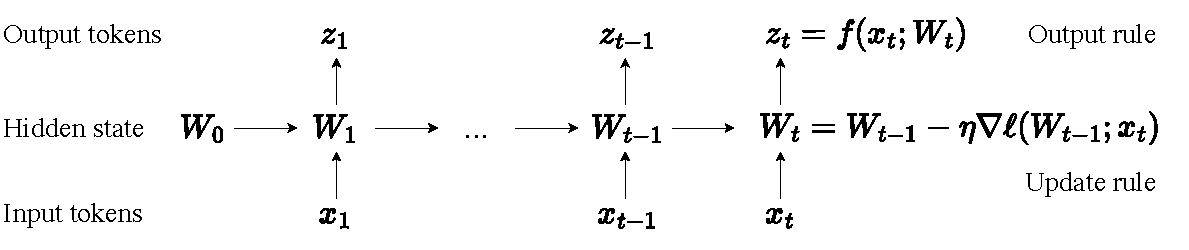
\includegraphics[width=0.8\textwidth]{figs/simple_teaser.pdf}
    \caption{All RNN layers can be expressed as a hidden state that transitions according to an update rule.
    The key idea in \cite{sun2024ttt} is to make the hidden state itself a model $f$ with weights $W$, and the update rule a gradient step on the self-supervised loss $\ell$.
    Therefore, updating the hidden state on a test sequence is equivalent to training the model $f$ at test time. 
    This process, known as Test-Time Training (TTT), is programmed into TTT layers. 
    Figure and caption taken from \cite{sun2024ttt}.
    }
    \label{fig:ttt-layer}
\end{figure*}

Despite the remarkable progress in visual and physical realism, state-of-the-art video Transformers are still generating mostly short clips of single scenes without complex stories.
At the time of writing (March 2025), the maximum length of public APIs for video generation is 20 seconds for Sora (OpenAI), 16 seconds for MovieGen (Meta), 10 for Ray~2 (Luma), and 8 for Veo~2 (Google).
None of these APIs can autonomously generate complex multi-scene stories.

A fundamental challenge behind these technical limitations is long context, because the cost of self-attention layers in Transformers increases quadratically with context length.
This challenge is especially acute for video generation with dynamic motion, whose context cannot be easily compressed by a tokenizer.
Using a standard tokenizer, each of our one-minute videos requires over 300k tokens in context. 
With self-attention, generating a one-minute video would have taken $11\times$ longer than generating 20 videos of 3 seconds each, and training would have taken $12\times$ longer.

To address this challenge, recent work on video generation has investigated RNN layers as an efficient alternative to self-attention, because their cost increases linearly with context length~\cite{wang2024lingenhighresolutionminutelengthtexttovideo}.
Modern RNN layers, especially variants of linear attention~\cite{schmidhuberlinearattn, katharopoulos2020lineartransformers} such as Mamba~\cite{gu2024mamba, dao2024mamba2} and DeltaNet~\cite{schlag2021deltanet, yang2025gateddeltanetworksimproving}, have shown impressive results for natural language tasks.
However, we have yet to see long videos with complex stories or dynamic motion generated by RNNs.
Videos (\href{https://lineargen.github.io/}{link}) in \cite{wang2024lingenhighresolutionminutelengthtexttovideo} are high resolution and one-minute long, but contain only single scenes and slow motion, let alone complex stories.

We believe that these RNN layers generate less complex videos because their hidden states are less expressive.
RNN layers can only store past tokens into a hidden state of fixed size, which is only a matrix for linear attention variants such as Mamba and DeltaNet.
It is inherently challenging to compress hundreds of thousands of vectors into a matrix with only thousands in rank.
As a consequence, these RNN layers struggle to remember the deep relationships between distant tokens.

We experiment with an alternative class of RNN layers whose hidden states themselves can be neural networks. Specifically, we use two-layer MLPs with 2$\times$ more hidden cells and richer nonlinearities than the linear (matrix) hidden states in linear attention variants.
Since the neural network hidden states are updated by training even on test sequences, these new layers are called Test-Time Training (TTT) layers~\cite{sun2024ttt}.

We start from a pre-trained Diffusion Transformer (CogVideo-X 5B \cite{hong2023cogvideo}) that could only generate 3-second short clips at 16 fps (or 6 seconds at 8 fps).
Then, we add TTT layers initialized from scratch and fine-tune this model to generate one-minute videos from text storyboards. 
We limit the self-attention layers to 3-second segments so their cost stays manageable.
With only preliminary systems optimization, our training run takes the equivalent of 50 hours on 256 H100s.

We curate a text-to-video dataset based on $\approx$ 7 hours of \textit{Tom and Jerry} cartoons with human-annotated storyboards.
We intentionally limit our scope to this specific domain for fast research iteration.
As a proof-of-concept, our dataset emphasizes complex, multi-scene, and long-range stories with dynamic motion, where progress is still needed; it has less emphasis on visual and physical realism, where remarkable progress has already been made.
We believe that improvements in long-context capabilities for this specific domain will transfer to general-purpose video generation.

Compared to strong baselines such as Mamba 2~\cite{dao2024mamba2}, Gated DeltaNet~\cite{yang2025gateddeltanetworksimproving}, and sliding-window attention layers, TTT layers generate much more coherent videos that tell complex stories with dynamic motion, leading by 34 Elo points in a human evaluation of 100 videos per method.
For context, GPT-4o scores 29 Elo points over GPT-4 Turbo in LMSys Chatbot Arena~\cite{chiang2024chatbot}.

Sample videos, code and annotations are available at:
\url{https://test-time-training.github.io/video-dit}
\section{Related Works}
\label{sec:related_works}

\noindent \textbf{Video large language models}.
Recent advances in instruction tuning with visual and text data~\cite{liu2023visualinstructiontuning, liu2023improvedllava, liu2024llavanext} have led to a surge of interest in developing Video LLMs. Many of these models share a common design, where visual features are extracted using a pre-trained visual encoder, projected into the text latent space of an LLM, and subsequently processed by the pre-trained LLM to generate responses. 
%
Video-ChatGPT~\cite{maaz2024videochatgptdetailedvideounderstanding} introduces instruction tuning into the video domain. Video-LLaVA~\cite{lin2023video} improves model performance with better text-aligned video features \cite{zhu2023languagebind}, while VideoChat2~\cite{li2023mvbench} resorts to increasing the quality and quantity of the video instruction tuning set. Recent vision-LLM models like LLaVA-NeXT~\cite{liu2024llavanext}, LLaVA-OneVision~\cite{li2024llava}, LLaVA-Video~\cite{zhang2024videoinstructiontuningsynthetic}, Qwen2-VL~\cite{Qwen2VL}, and mPlug-Owl3~\cite{ye2024mplugowl3longimagesequenceunderstanding} consider multi-stage training with both video and image, which substantially improves the model performance.
Recent works in VideoLLM focus on long video understanding. ~\cite{wang2024videollamblongcontextvideounderstanding, faure2024hermestemporalcoherentlongformunderstanding, weng2024longvlmefficientlongvideo, korbar2024textconditionedresamplerlongform, zhang2024longcontexttransferlanguage, shen2024longvu} propose to use Q-former~\cite{li2023blip2bootstrappinglanguageimagepretraining} or text-query-based cross-attention to compress vision tokens, while others~\cite{nguyen2024encodingcontrollingglobalsemantics, wang2024longllavascalingmultimodalllms} resort to state-space models~\cite{gu2024mambalineartimesequencemodeling}.
Researchers also extend the instructional tuning into different video sub-domains. For instance, CAT~\cite{ye2024catenhancingmultimodallarge} focuses on audio-visual understanding, while Scene-LLM~\cite{fu2024scenellmextendinglanguagemodel} and LLaVA-3D~\cite{zhu2024llava3dsimpleeffectivepathway} address 3D QA tasks.

Built on these developments, our work specifically focuses on adapting pre-trained Video LLMs to downstream tasks with side-channel signals, aiming to significantly extend the capabilities of these models. 

%LLaVA proposes visual instruction tuning which extended instruction tuning to computer vision and create the first vision-LLM. Subsequent research focus on create a better visual representation by increasing the input resolution \cite{liu2023improvedllava, liu2024llavanext} and developing higher-quality large-scale instruction tuning data \cite{li2024llava}. 

%While all these models need large scale pre-training with video instruction tuning set or task-special training set. Our works focus on adapting the existing Video LLM trained in the general video understanding to different video down-stream tasks efficiently.

% Yin: I have to re-write the following sub-section. 
\medskip
\noindent \textbf{Adaptation of vision foundation models}. Adapting vision foundation models to downstream tasks has received significant attention. Prior works have studied learning lightweight adapters~\cite{rebuffi2017learning,lian2022scaling,bhattacharjee2023vision,chen2022adaptformer,sung2022vl,chen2023vision}, prepending learnable input tokens (\eg prompts)~\cite{zhou2022learning,jia2022visual}, or in-context learning~\cite{wang2023images,xu2024towards,bar2022visual,zhang2023makes}. Recently, adapter- and prompt-based methods have been explored for Video LLMs. Adapt2Reward~\cite{yang2024adapt2reward} re-purposes a video-language model for robotic operation by using it as a language-conditioned reward function. Similarly, SeViLA~\cite{yu2024self} adapts an image-language model for video tasks by introducing Localizer and Answerer modules, derived from BLIP-2~\cite{li2023blip2bootstrappinglanguageimagepretraining}, to enable video event localization and question answering.

Our work is inspired by the success of adapter-based methods such as LoRA~\cite{hu2021loralowrankadaptationlarge}. These methods learn parameter-efficient modules without changing the base model's architecture and weights, and has been widely used to customize large, pre-trained diffusion models for image generation~\cite{kumari2022multiconcept,xiao2023fastcomposer,gu2023mixofshow,wang2023autostory,shah2023ziplora,zhong2024multi}, extending their capabilities in generating images with different styles or controlling the generated content. Moving beyond diffusion models, our goal is to offer a flexible framework that adapts Video LLMs to a wide range of tasks with patch-like adapters, allowing these models to effectively account for additional side-channel signals and adapt to downstream tasks.


%On the other hand, some techniques, such as LoRA~\cite{hu2021loralowrankadaptationlarge} can be widely used to customize foundation models in different settings. These LoRA adapters are first proposed in adapting LLMs and offer a patch to the base model by adding a small number of parameters and operations, without changing the base model's architecture and weights. Similar ideas have recently been embraced by the vision community. For example, patch-like adapters~\cite{kumari2022multiconcept,xiao2023fastcomposer,gu2023mixofshow,wang2023autostory,shah2023ziplora,zhong2024multi} have been designed to customize large, pre-trained diffusion models for image generation, significantly extending their capabilities in generating images with different styles or controlling the generated content. 

%Motivated by this line of research, instead of focusing on adapting the Video LLM to a specific setting, PAVE aims to offer a framework that adapts Video LLMs to a wide range of tasks with a patch-like adapter, allowing these models to effectively account for additional side-channel signals and adapt to downstream tasks.

\medskip
\noindent \textbf{Multimodal video representation learning}.
Learning a unified representation to connect video and other modalities, such as audio, text and point cloud, has received considerable attention. Prior methods~\cite{luo2022clip4clip} build on the idea of modality alignment using contrastive learning~\cite{radford2021learningtransferablevisualmodels}. More recent works~\cite{chen2023valor, chen2023vast,zhang2023meta,girdhar2023imagebind,zhu2023languagebind} extend the alignment across multiple modalities. Inspired by these works, our method leverages the shared representation between video and text learned by a pre-trained Video LLM, and further embeds side-channel signals into this latent space during adaptation. %Instead of a global video representation, our model aligns key video frames with side-channel signals in time, and matches patch-level vision tokens to those from side-channel signals, 


%Our key technical  aligns the video with the side-channel signals in time, and 


%A key design choice is when to fuse information from video and other modalities. Late fusion has been widely adopted by representation learning methods~\cite{luo2022clip4clip,chen2023valor, chen2023vast,zhang2023meta,girdhar2023imagebind,zhu2023languagebind}, where the video and other modality representations are separately encoded and later aligned in a shared latent space. This is, however, in contrast to many cross-modal video understanding models, which fuse video and other signals at the initial stage of processing~\cite{xu2019multilevel,zhang2019man}. Indeed, a few recent works find early fusion helpful to strengthen cross-modal reasoning~\cite{mo2024unveiling,barnum2020benefits}. 




%and further map supplementary information into this share semantic space during the adaptation. 



%CLAP \citep{laionclap2023} focus on audio and text representation learning, and PointCLIP \citep{zhang2022pointclip} aligns point clouds with text.

%VALOR \citep{chen2023valor} and VAST \citep{chen2023vast}, extending the alignment process with additional modalities can enhance the model's robustness while maintaining its performance. Meta-transformer \citep{zhang2023meta} supports 12 different modalities and employs unique tokenizers to unify the embedding space across these modalities. ImageBind \citep{girdhar2023imagebind} expands multi-modal alignment pretraining to encompass six modalities. LangugeBind~\cite{zhu2023languagebind} builds a multi-modal representation among 5 different modalities by treating all modalities as image.


%Multi-modal representation learning started with pretraining using both vision and language data. CLIP \citep{radford2021learningtransferablevisualmodels} initiates image-text representation learning by training on 400M text-image paired, effectively connecting these two domains and build a shared representation. Additionally, CLIP serves as a foundation for building up the representation in other modalities. For example, CLIP4Clip \citep{luo2022clip4clip} builds the shared representation between video and text, CLAP \citep{laionclap2023} focus on audio and text representation learning, and PointCLIP \citep{zhang2022pointclip} aligns point clouds with text.

%More recent effort aims to building the unified representation across multiple modalities.  Observed in VALOR \citep{chen2023valor} and VAST \citep{chen2023vast}, extending the alignment process with additional modalities can enhance the model's robustness while maintaining its performance. Meta-transformer \citep{zhang2023meta} supports 12 different modalities and employs unique tokenizers to unify the embedding space across these modalities. ImageBind \citep{girdhar2023imagebind} expands multi-modal alignment pretraining to encompass six modalities. LangugeBind~\cite{zhu2023languagebind} builds a multi-modal representation among 5 different modalities by treating all modalities as image.





%to adapt large-scale pre-trained diffusion models for image generation tasks. 

%Foundation models are defined by their ability to adapt to a wide range of downstream tasks. Specifically, in natural language processing (NLP) domain, Large language Models (LLM) \cite{chatgpt, gpt4, llama3_2} trained with large scale dataset has strong zero-shot ability on different Natural Language Processing (NLP) tasks. With instruction tuning \cite{brown2020language, ouyang2022training, wang2022benchmarking, wang2022self} human further adapt and align the pretrained LLM with human interests and improve the model performance on different down-stream task. 

%In computer vision domain, an example of foundation model adaptation is the concept customization of diffusion model. 
%Custom Diffusion~\cite{kumari2022multiconcept} fine-tunes the model on  multiple concept images for customization.
%To expedite customized generation, FastComposer~\cite{xiao2023fastcomposer} fine-tunes a diffusion model on a substantial amount of data, enabling it to take subject embeddings as input and create composed images featuring multiple concepts. Given the extensive use of LoRA for customization, several recent studies~\cite{gu2023mixofshow,wang2023autostory,shah2023ziplora,zhong2024multi} aim to achieve multi-concept customization by merging multiple LoRA weights associated with individual concepts.

%While instruction tuning in NLP and adding LoRA adapter for adapting the diffusion model only take input from same modality as the original model. PAVE aims adapt the Video LLM into a new setting with supplementary information.  

% Video understanding is a long-standing problem and it has many well-defined subdomains. For instance, video question answering\cite{le2020hierarchical} and Video Action Recognition\cite{feichtenhofer2016convolutional} aims to understand the human action appear in the video, temporal action localization\cite{zhang2022actionformer} detect the interested the actions and localize the event along the temporal axis, video grounding\cite{zeng2020dense, mu2024snagscalableaccuratevideo} find the temporal interval given the questions, captioning\cite{wang2018reconstruction} for generating the text description for the video,  video anticipation\cite{furnari2020rolling} to anticipate the actions the action in the following moments.

% To improve the model performance on different video tasks, finding a better video representation is a ever-lasting research topic.
% Two-Stream Network\cite{feichtenhofer2016convolutional} are well explored in the traditional video understanding task, Slow-fast\cite{feichtenhofer2019slowfastnetworksvideorecognition},TSP\cite{alwassel2021tsp}
% I3D\cite{carreira2018quovadisactionrecognition}. They propose different two stream network to complementary with each other. Specifically, the Slow-Fast Network combine the fast path which captures the motion information from temporal densely sampled video frames with the slow path which encodes the static vision semantic information from high spatial resolution frames.

% Our model inspired by the idea of the Slow-Fast Network. Instead of flatten all the information in slow path and fast path and combine them by concatenation. We use Cross-attention to absorb the information from the fast-path to the slow-path. By explicitly considering the spatial-temporal alignment, we are able to extend the length of the fast path to large number instead of restricted by a fixed scaling factor.



\begin{figure*}[t]
    \centering
    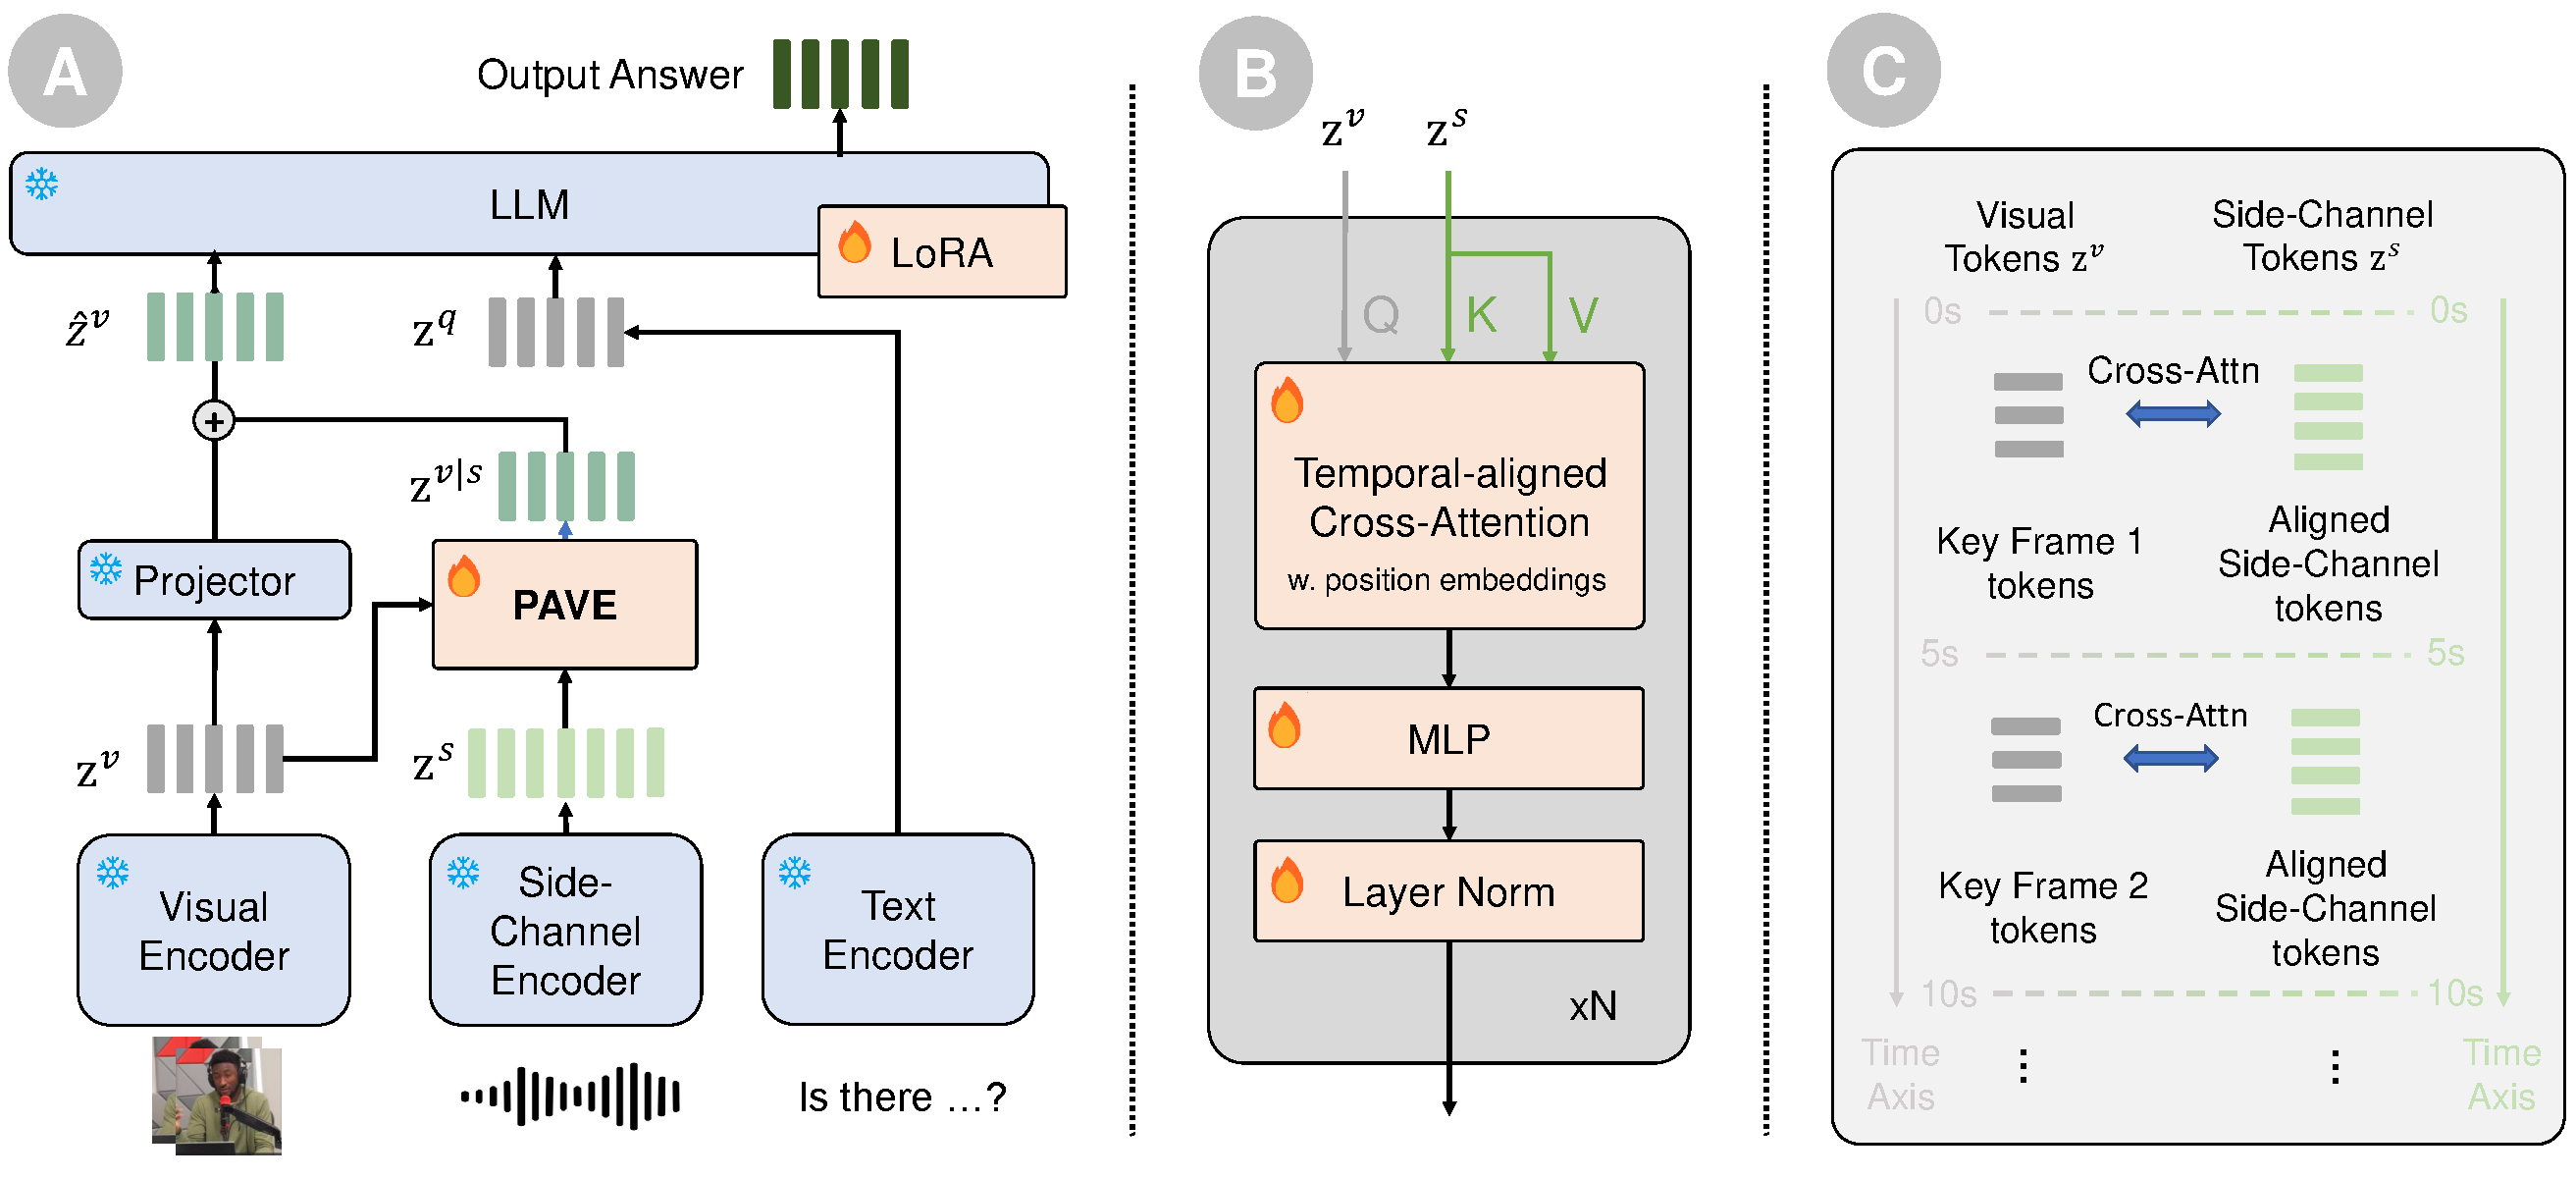
\includegraphics[width=0.85\linewidth]{new_figure_source/pave_overview_updated.pdf}
    \vspace{-0.5em}
    \caption{(a) \textbf{Overview of PAVE}. PAVE presents a simple, parameter-efficient adapter to integrate videos and side-channel signals. This is done by fusing side-channel tokens $\mathbf{z}^s$ and video tokens $\mathbf{z}^v$, and further adding the results to the original video tokens $\mathbf{z}^v$.  (b) \textbf{Details of PAVE's fusion function}. The fusion function $g(\cdot)$ consists of a few blocks of temporal-aligned cross-attention layer, MLP, and layer normalization. (c) \textbf{Temporal-aligned Cross-Attention}. Visual tokens $\mathbf{z}^v$ and side-channel tokens $\mathbf{z}^s$ are aligned along the temporal axis. A video token $\mathbf{z}^v(k)$ is treated as query, and only attends to keys and values (defined by side-channel tokens) in its temporal neighborhood.}
    \label{fig:structure_overview}
    \vspace{-1em}
\end{figure*}

\section{Patching and Adapting Video LLMs}
\label{sec:method}

% ovewview paragraph
We propose \textbf{PAVE}, a framework for adapting pre-trained Video LLMs to downstream tasks with side-channel signals. The key to our solution lies in a parameter-efficient, lightweight adapter, referred to as a patch. 
%only introduces a small number of parameters and operations and 
This patch fuses side-channel signals with the original visual tokens and updates them (see Figure~\ref{fig:structure_overview} (a)), and adds a LoRA module~\cite{hu2021loralowrankadaptationlarge} to the LLM, enabling efficient adaptation with a small number of parameters and operations and without altering the base model. 
%Additionally, we fine-tune the LLM using LoRA~\cite{hu2021loralowrankadaptationlarge}, enabling efficient adaptation through patching.
% ---
In what follows, we introduce the background on Video LLM, outline our problem formulation, and present our approach.
%and further describe the implementation details.   

%we present \textbf{PAVE}, a framework designed to \underline{P}atch and \underline{A}dapt \underline{V}id\underline{e}o LLMs. PAVE leverages a variant of cross-attention mechanism that operates between tokens derived from key video frames (as queries) and tokens from side-channel signals (as keys and values). This operations seeks to align the video frames and side-channel signals along the time axis, fuse the signals from both sources, and then update the input visual tokens to the LLM. In doing so, PAVE allows for the input of supplementary signals, and introduces a small number of parameters and operations with a negligible memory footprint and computing cost, while enabling effective adaptation to various downstream tasks without altering pre-trained models.


\subsection{Preliminaries: Video LLM}
A Video LLM takes a video $\mathbf{X}^v$ and a text query $\mathbf{X}^q=\{x^q\}$ as input, then generates a text answer $\mathbf{X}^a=\{x^a\}$. We assume that $\mathbf{X}^v = \{\mathbf{X}^v_1, \mathbf{X}^v_2, ..., \mathbf{X}^v_K\}$, \ie, a video is represented by $K$ key frames, where $K$ may vary across videos. $\mathbf{X}^v$ is first encoded by a visual encoder
% (including the vision backbone and its projector) 
$h_v(\cdot)$ into a set of visual tokens $\{\mathbf{z}^v(k) \in \mathbb{R}^{M \times d}\}$, where $\mathbf{z}^v(k)$ indicates $M$ tokens encoded from the $k$-th key frame within the video ($k \in [1, K]$). Similarly, $\mathbf{X}^q$ is processed by a text encoder $h_t(\cdot)$, which embeds individual words $x^q$ into text tokens $\{\mathbf{z}^q \in \mathbb{R}^d\}$ with $\mathbf{z}^q = h_t(x^q) $. 
These tokens are further combined and processed by an LLM $f(\cdot)$ that decodes $\mathbf{X}^a$ in an autoregressive manner
\begin{equation}
    f\left( \left[ \{\mathbf{z}^v(k)\}, \{\mathbf{z}^q\}, \{\mathbf{z}^a_{<i}\} \right]; \mathbf{\theta} \right) \rightarrow x_i^a, \label{eq:llm}
\end{equation}
where $\{\mathbf{z}^a_{<i}\}$ are text tokens from previously generated answer $x^a_{<i}$, \ie, $\mathbf{z}^a = h_t(x^a)$. $\mathbf{\theta}$ denotes LLM parameters. 

\subsection{Video Tasks with Side-Channel Signals}
% problem formulation / use cases
We consider adapting a pre-trained Video LLM to downstream tasks with side-channel signals $\mathbf{X}^s$. Similar to videos, we assume that $\mathbf{X}^s = \{\mathbf{X}^s_1, \mathbf{X}^s_2, ..., \mathbf{X}^s_{K_s}\}$, \ie, the side-channel signals also follow a temporal order and are split into $K_s$ blocks. We additionally assume a separate encoder (with possible projector) $h_s(\cdot)$ to process $\mathbf{X}^s$ into a collection of tokens $\{\mathbf{z}^s(k_s) \in \mathbb{R}^{M' \times d} \}$, where $\mathbf{z}^s(k_s)$ is $M'$ tokens encoded from the $k_s$-th block of the side-channel.  It is worth noting that this formulation encapsulates a range of video tasks. We describe some of these tasks considered in our experiments. 

\begin{itemize}
    \item \textbf{Audio-visual understanding}. This task requires jointly processing video and its accompanying audio data (as side-channel signals) for scene understanding, such as event recognition~\cite{xiao2020audiovisual} or QA~\cite{alamri2019audiovisualsceneawaredialog}. 
    \item \textbf{3D scene understanding}. This task focuses on reasoning about the 3D scene using a video of a 3D scan~\cite{azuma_2022_CVPR}. Camera trajectories, as well as an optional sequence of depth maps, constitute the side-channel signals.  
    \item \textbf{Multi-view video understanding}. This task involves combining multi-view videos for visual recognition, \eg, using exocentric videos to complement egocentric video for understanding human activities~\cite{grauman2024ego}. 
    \item \textbf{Enhancing video representations}. This task seeks to enhance the visual representation in the Video LLM. This is done by integrating low resolution, high frame rate frames with the original input of high resolution, low frame rate frames, following the key idea of SlowFast networks~\cite{feichtenhofer2019slowfastnetworksvideorecognition}.

\end{itemize}

\subsection{Our Design of PAVE}
% the key idea: x-attention for fusion and summation for aggregation; technical details about temporal alignment / positional encoding

Our goal is to integrate side-channel signals $\mathbf{X}^s$ into the LLM to enhance video reasoning, without modifying the structure of $f(\cdot)$ and encoders ($h_v(\cdot)$ and $h_t(\cdot)$), nor adding any major set of parameters. To achieve this goal, our key idea is learning a function $g(\cdot)$ to fuse side-channel tokens $\{\mathbf{z}^s(k_s)\}$ with the original visual tokens $\{\mathbf{z}^v(k)\}$. The fusion results have the same size of $\{\mathbf{z}^v(k)\}$, and will be further used to update $\{\mathbf{z}^v(k)\}$. Formally, our design of PAVE, as shown in Figure~\ref{fig:structure_overview} (a), is expressed as
\begin{equation}
\begin{split}
    \text{fusion:} \quad & \{\mathbf{z}^{v|s}(k)\} = g([\{\mathbf{z}^s(k_s)\}, \{\mathbf{z}^v(k)\}]; \phi)\\
    \text{summation:} \quad & \mathbf{\hat{z}}^{v}(k) = \mathbf{z}^{v}(k) + \mathbf{z}^{v|s}(k),
\end{split}\label{eq:pave}
\end{equation}
where $\phi$ denotes learnable parameters of $g(\cdot)$. 

Intuitively, $g(\cdot)$ injects side-channel information into a set of tokens of the same size as the original visual tokens, based on which a simple summation can be performed to form a residual connection. A key feature of this design is that the number of input tokens to $f(\cdot)$ remains unchanged. As the main computational cost lies in $f(\cdot)$, doing so results in a negligible overhead. 

\medskip
\noindent \textbf{The fusion function $g(\cdot)$}. Our fusion function is realized using a variant of cross-attention, as illustrated in Figure~\ref{fig:structure_overview} (b). Specifically, the vision tokens $\{\mathbf{z}^v(k)\}$ are transformed into the queries, and the side-channel tokens $\{\mathbf{z}^s(k_s)\}$ form the keys and values. To align video and side-channel signals in time while maintaining a low computation cost, we consider a local cross-attention, named temporal-aligned cross-attention, where a query $\mathbf{z}^v(k)$ only attends to keys and values in its temporal neighborhood, \ie, $\{\mathbf{z}^s(k_s)\}$ with $k_s \in N(k)$ (see Figure~\ref{fig:structure_overview} (c)). Before computing the cross attention, rotary positional embeddings~\cite{su2024roformer} are added to the queries and keys. After cross attention, an MLP with layer normalization is applied to further transform the features, similar to a standard Transformer block~\cite{vaswani2017attention}.


\medskip
\noindent \textbf{Integration with LoRA and training loss}. We further combine PAVE with LoRA~\cite{hu2021loralowrankadaptationlarge} by adding a small set of parameters in the form of low rank approximation $\Delta \theta$ to the LLM $f(\cdot)$. Putting things together, PAVE minimizes the standard negative log likelihood of its output when adapting to a downstream task. This is given by 
\begin{equation*}
\argmin_{\mathbf{\Delta\theta}, \mathbf{\phi}} \ \mathbb{E}_{\mathcal{D}} \ \left[ -\log p \left( x^a_i | \left[ \{\mathbf{\hat{z}}^{v}\}, \{\mathbf{z}^{q}\}, \{\mathbf{z}^a_{<i}\} \right]; \theta+\Delta \theta, \phi \right) \right],
\end{equation*}
where $\mathcal{D}$ is the data distribution approximated by the training set $(\mathbf{X}^v, \mathbf{X}^q, \mathbf{X}^a) \sim \mathcal{D}$. $\{\mathbf{\hat{z}}^{v}\}$ is computed using Eq.\ \ref{eq:pave}, thus creating a dependency on $g(\cdot)$ and its parameters $\phi$.
%The learnable parameters thus include the LoRA parameters $\Delta \theta$ in $f(\cdot)$, and the parameters $\phi$ in $g(\cdot)$ 

%A simple solution is given by LoRA~\cite{hu2021loralowrankadaptationlarge}. It learns a small set of parameters in the form of low rank approximation $\Delta \theta$. However, this solution does not allow us to make use of $\mathbf{X}^s$. 

% \subsection{Implementation Details}
% % all other things including some of the implementation details.
% Inside the attention layer, we add rotary position embedding to the query and key tokens. Specifically, we apply different rotary positional embedding according to the layout of side-channel tokens $\mathbf{z}^s$. We mainly consider two types of $\mathbf{z}^s$: (a) $\{\mathbf{z}^s\}$ includes both spatial and temporal dimensions, such as tokens from video backbones or from 3D backbone; and (b) $\{\mathbf{z}^s\}$ only contains temporal dimension, such as audio tokens. For the first case, we will add 3D rotary positional embedding (along the temporal, height, and width dimensions). For the second case, we will only add rotary positional embedding along the temporal axis. After cross-attention, we use a two-layer MLP, followed by a layer norm. We initialize the $\gamma$ in the layer norms to zero. For all experiments, we use a learning rate of 2e-5 and a batch size of 32 to adapt the pre-trained Video LLM.


\begin{comment}
\subsection{Background}
Current video Large Language Models (Video LLMs) have three components: Visual Encoder, Projector, and Language Model (LM).

\noindent\textbf{Visual Encoder.} It encodes the vision input into a latent feature space. The common choices for the vision encoder are ViT\cite{dosovitskiy2021imageworth16x16words} from CLIP\cite{radford2021learningtransferablevisualmodels}, SigLIP \cite{zhai2023sigmoidlosslanguageimage}, and multi-modality encoder LanguageBind\cite{zhu2023languagebind}. The encoded feature will be delivered to the adapter. We call features from the vision encoder as original visual tokens, $V_{origin}$.


\noindent\textbf{Projector.} The projector is the module convert the vision feature to the text latent space. In many recent research\cite{tong2024cambrian1fullyopenvisioncentric, liu2024llavanext} shows that the 2 layers MLP is strong enough to bridge the domain gap. We name the feature converted by after the projector as projected visual tokens, $V_{projectored}$

\noindent\textbf{Language Model.} The language model will process projected vision information and the questions to give an answer. The popular choice for the language model are Llama\cite{touvron2023llama2openfoundation,llama3_2}, Vicuna\cite{vicuna2023}, and Qwen-2\cite{yang2024qwen2technicalreport}.


\subsection{PAVE structure}
The overview of the PAVE structure is shown on the left panel of figure~\ref{fig:structure_overview}. For specific downstream tasks, the high level idea of PAVE is to create a 'Patch' and attach it to the Video LLM without altering the original model parameters and adapt the Video LLM into a new setting. This patch collects the task-specific additional information and add it back to the adapted visual tokens $V_{adapted}$, using a residual connection. 

\noindent\textbf{Input of the PAVE.} PAVE’s input has two sources: original visual tokens, $V_{origin}$, from the Video LLM's vision encoder, and the other is task-specific tokens $T$ from the encoder which encode the task-specific additional information.

\noindent\textbf{Temporal Alignment Module}
Given the fact that, the task-specific tokens $T$ and original visual tokens $V_{origin}$ may have different temporal granularities. Considering that temporally close visual and additional information are strongly correlated, as they jointly represent the same scene, we use temporal alignment module to explicit align them. This approach not only reduces noise introduced by temporal misalignment but also further reduces computational resource needed in cross-attention.

To do this we first split the task-specific tokens $T$ and original visual tokens $V_{origin}$ based on their smallest temporal unit, respectively. We then have $T = \{T_0, T_1, ... , T_n\}$ and $V_{origin}=\{V_0, V_1, ... , V_m\}$. For instance, if input of the Video LLM's vision encoder consist of 32 frames, then original visual tokens $V_{origin}$ should be split into $\{V_0, V_1, ... , V_{31}\}$. We always use the $\{V_0, V_1, ... , V_m\}$ as anchors on the temporal axis and evenly divide the $\{T_0, T_1, ... , T_n\}$ into $m$ groups.


\begin{align*}
\{T_0, T_1, \dots, T_n\} &= \Big\{ \{T_{00}, T_{01}, \dots, T_{0k}\}, \\ 
                          &\quad \{T_{10}, T_{11}, \dots, T_{1k}\}, \dots, \\ 
                          &\quad \{T_{m0}, T_{m1}, \dots, T_{mk}\} \Big\}
\end{align*}


For some special case that $\{T_0, T_1, ... , T_n\}$ could not be evenly split into m groups, we will pad the group which lengthen is smaller than $\ceil*{\frac{n}{m}}$. Right panel of figure~\ref{fig:structure_overview} show the visualization of temporal alignment module. We then pair the $V_i$ with $\{T_{i0}, T_{i1}, \dots, T_{ik}\}$ as mini-batch $mbatch_i = (V_i, \{T_{i0}, T_{i1}, \dots, T_{ik}\})$ and create $m$ mini-batches in total.

\noindent\textbf{Cross-Attention Module and 3-dimension Rotary Positional Embedding.}
After Obtaining the $m$ mini-batches from the Temporal Alignment Module we conduct cross-attention within each mini-batch, Where $V_i$ will be the query and $\{T_{i0}, T_{i1}, \dots, T_{ik}\}$ will be the key. Thus it aggregate the additional information from $\{T_{i0}, T_{i1}, \dots, T_{ik}\}$ into $V_i$ and and yield a group of updated tokens $V_{updated}=\{V_{updated_0}, V_{updated_1}, ... , V_{updated_m}\}$

During the cross-attention, We mainly consider two types of task-specific tokens $T$ : 1. tokens $T$ with spatial dimensions, such as video tokens from video backbones and 3D tokens from 3D backbone, 2. tokens $T$ without spatial dimensions, such as audio tokens. For the first case we will add 3 dimension rotary positional embedding along the temporal, height and width dimension. For the second case we will only add rotary positional embedding along the temporal axis.

\noindent\textbf{Zero-Initialized Residual Connection.}  After aggregating all additional information into $V_{updated}$, $V_{updated}$ will pass through an MLP and a Layer Normalization layer. Specifically, we initialize the $\gamma$ in layer norm to zero, this will ensure that the beginning of the training PAVE module will not have any effect on the Video LLM. 
Finally we add up $V_{updated}$ with the projected visual tokens $V_{projected}$. The $V_{adaptored} = V_{updated} + V_{projected}$ will be sent into the LLM for reasoning.

\subsection{The Training of PAVE}
In the PAVE, the Cross-Attention layers, the MLP and the layer normalization layer are trainable, while other modules remain forzen. During the adaptation, we also apply LoRA to the LLM to adapt the LLM for making use of the additional information.
We use the original auto-regressive training objective to train the PAVE, specially for a sequence of length L, we maximize the probability of the target answers $\mathbf{X}_\text{a}$ during the adaptation by:
\begin{align*}
        p(\mathbf{X}_\text{a} \mid V_{adaptored}, \mathbf{X}_\text{instruct}) = \\
    \prod_{i=1}^{L} p_\theta (x_i \mid V_{adaptored}, \mathbf{X}_\text{instruct, $<$ i}, \mathbf{X}_\text{a, $<$ i})
\end{align*}
where, the $\mathbf{X}_\text{a}$ is the target answer, $V_{adaptored}$ is the PAVE adapted visual features, $\mathbf{X}_\text{instruct}$ is the question and instruction, and $\theta$ represent the all trainable parameters.
\end{comment}
\section{Experiments and Results}\label{sec:experiments}
Our main experiments include (1) audio-visual QA (Sec.\ \ref{section_res_audio}), (2) 3D QA (Sec.\ \ref{section_res_3d}, (3) enhancing video QA by considering high frame rate videos (Sec\ \ref{section_res_video}), and (4) multi-view video recognition (Supplement). In addition, we ablate our design, investigate cross-model generalization, and demonstrate multi-task joint training in Sec.\ \ref{section_res_ablation}. Further implementation details for individual experiments can be found in the Supplement.  

%an ablation study of our method in Sec~\ref{section_res_ablation}, and the result of multi-view video understanding in the Appendix.
%We also includes the multi-view video understanding by supplementing ego-centric video with exo-centric video in Appendix Sec~\ref{section_res_multi_view_video}.
% Finally, We also include the multi-view video understanding by supplementing ego-centric video with exo-centric video in Appendix.


\begin{table*}[t]  
\centering  
\scalebox{0.7}{
\begin{tabular}{lc|c|cccc|c|c}  
\toprule
       \multirow{2}{*}{Method}      & AVSD~\cite{alamri2019audiovisualsceneawaredialog}  &AVQA~\cite{yang2022avqa}&\multicolumn{4}{c|}{MUSIC-AVQA~\cite{Li2022Learning}}  & \multirow{2}{*}{TFLOPs} & \multirow{2}{*}{Total / Trainable Params} \\
                                    & CIDEr                                              & Acc. &Audio Acc. & Visual Acc. & Audio-Visual Acc.  & Overall Acc. & & \\
    \midrule
    \multicolumn{3}{l}{\it \small\textbf{Zero-shot LMMs} } \\
     CAT-7B ~\cite{ye2024catenhancingmultimodallarge}             & 79.0 & -  & -  & -    & -    & 48.6 & -      & - \\
     %LLaVA-OV-0.5B~\cite{li2024llava}                            &  65.1 & 0.9B~/~-\\
     LLaVA-OV-7B~\cite{li2024llava}                               & 70.6 & 85.6  & \textcolor{gray}{68.8} & 70.6 & 52.8 & 60.4 & 98.53 & 8.2B~/~-\\
     \midrule
     \multicolumn{3}{l}{\it \small\textbf{Task-specific models} } \\     
     MTN~\cite{Le_2019}                                           & 98.5  & -  & - & - & -  &  - &-  & -\\
     COST~\cite{pham2022videodialogconversationobjects}           & 108.5 & -  & - & - & -  &  - &-  & - \\
     VALOR~\cite{chen2023valor} & -  & - & - & -  & -&  78.9 & - & - \\
     VAST~\cite{chen2023vast} & -  & - & - & -  & -&  80.7 & - & - \\
     PSTP-Net~\cite{li2023progressive} & -  & 90.2 & - & -  & -&  - & - & - \\
     CAT-7B-FT ~\cite{ye2024catenhancingmultimodallarge}          & - & 92.0 & \textcolor{gray}{\textbf{84.9}} & 86.1 & \textbf{83.2} &    \textbf{84.3} & -  & - \\ %0.6492%
     LLaVA-OV-7B-FT                                               & 124.9 & 90.8 & \textcolor{gray}{75.4} & 89.3 & 72.3 &  77.4  &98.53 & 8.2B~/~161.5M \\
     \midrule
     %Our-0.5B (fine-tuning)                                         &  117.6 & 0.9B~/~35.2M \\
     
     %Our-0.5B (w/ audio)                                          & \textbf{134.2}  & 0.9B~/~41.3M   \\
     PAVE-7B   (w/ audio)                                          & \textbf{152.9} & \textbf{93.8} & \textcolor{gray}{79.7} & \textbf{93.0} & 78.0 &  82.3 & 98.63 & 8.2B~/~170.5M \\ \bottomrule

\end{tabular}
}
\vspace{-1mm}
\caption{\textbf{Results of audio-visual QA} with audio as side-channel signals. We report CIDEr scores on AVSD and the accuracy (Acc.) on AVQA and Music-AVQA. LLaVA-OV-7B-FT refers to directly fine-tuning the LLaVA-OneVision using video. \textcolor{gray}{Gray} indicates results that require audio-inference only. Our model achieves state-of-the-art performance on AVSD, AVQA and visual split of Music-AVQA by only adding a small amount of parameters and FLOPs.
\vspace{-4mm}
}  
\label{tab:video_audio_understanding}  
\end{table*}  

\subsection{Results on Audio-Visual QA} \label{section_res_audio}

Audio-visual QA aims to answer questions related to various visual and auditory concepts (\eg, objects and the sound they produce), as well as their interactions in videos, based on an input of video with its accompanying audio. In this task, we treat audio as the side-channel signals. We now describe our experiment protocol, implementation details, baselines, and results. 

% Yin: The motivation is not needed here, as we do not invent any of these tasks. A clear definition is more than sufficient. 

%\noindent\textbf{Motivation and task set up.} While video naturally includes audio, most existing Video LLMs do not utilize this information. We believe that combining video and audio inputs can enhance a model's understanding of video content while adapting Video LLMs to the audio-visual setting remains unexplored. In this section, we use PAVE to adapt Video LLM to this setting with audio as the side-channel.

\medskip
\noindent\textbf{Experiment protocol.} Our experiments consider both open-end QA (AVSD~\cite{alamri2019audiovisualsceneawaredialog}) and closed-end QA (AVQA~\cite{yang2022avqa} and Music-AVQA~\cite{Li2022Learning}). We follow the protocol in previous works~\cite{ye2024catenhancingmultimodallarge, pham2022videodialogconversationobjects} to train and evaluate PAVE using corresponding splits of the datasets. For the open-end AVSD, we use the AVSD@DSTC7 test split and report the CIDEr score as the metric. For the closed-end AVQA and Music-AVQA, we evaluate PAVE on the standard eval / test split, and report the accuracy as the metric. For PAVE, we additionally calculate the model inference FLOPs during prefilling, as well as the total / trainable number of parameters. 

%the open-end QA dataset AVSD~\cite{alamri2019audiovisualsceneawaredialog}, and closed-end QA dataset AVQA~\cite{yang2022avqa} and Music-AVQA~\cite{Li2022Learning} as training dataset. 
% We train PAVE with the AVSD / AVQA / Music-AVQA training set when evaluating PAVE performance on AVSD / AVQA / Music-AVQA, respectively. 
%We follow the protocol in previous works~\cite{ye2024catenhancingmultimodallarge, pham2022videodialogconversationobjects} to evaluate PAVE. 
%This benchmark consists of 1,000 audio-visual questions.
%We use COCO API~\cite{lin2015microsoftcococommonobjects} to calculate the CIDEr score. 
%For AVQA / Music-AVQA, we evaluate PAVE on the eval / test split, respectively, and report the accuracy as the metric. 
%Additionally, we calculate the model inference FLOPs at the prefilling stage using LLM-Viewer~\cite{yuan2024llm}.

\medskip
\noindent\textbf{Implementation details.} 
To encode audio we extract audio features using ImageBind~\cite{girdhar2023imagebind}. It samples the audio at a 16kHz rate, generating approximately 1 audio token per second. PAVE further integrate these audio tokens into a Video LLM (LLaVA-OneVision~\cite{li2024llava}). We follow the LLaVA-OneVision~\cite{li2024llava} to evenly sample 32 video frames from an input video.
We train PAVE 1 epoch with the AVSD / 2 epochs with AVQA / 2 epochs with Music-AVQA training set, respectively. We then evaluate PAVE's performance on their corresponding test set. 
% We train PAVE for 1 epoch on the AVSD and 2 epochs on the AVQA and Music-AVQA.

\medskip
\noindent\textbf{Baselines.}
We consider two types of baseline methods: 
(1) Multimodal LLMs designed for general video or audio-visual understanding, \eg, LLaVA-OneVision~\cite{li2024llava} and CAT~\cite{ye2024catenhancingmultimodallarge}, which have never been trained on the target dataset (\ie, zero-short inference); and 
(2) Task-specific models, which has been fine-tuned on the target dataset, such as MTN~\cite{Le_2019} and COST~\cite{pham2022videodialogconversationobjects} for AVSD, PSTP-Net~\cite{li2023progressive} and CAT-7B-FT~\cite{ye2024catenhancingmultimodallarge} for AVQA, and the VALOR~\cite{chen2023valor}, VAST~\cite{chen2023vast} and CAT-7B-FT for Music-AVQA. 
%
We also include a baseline that directly fine-tunes our base model (LLaVA-OneVision) with LoRA on the training set without using the audio, denoted as LLaVA-OV-7B-FT. 
% This baseline allows us to assess whether PAVE can effectively utilize supplementary information.

\begin{table*}[t]  
\centering  
\scalebox{0.75}{
\begin{tabular}{lccccc|c|c|c}  
\toprule
\multirow{2}{*}{Method}                                          & \multicolumn{5}{c|}{ScanQA~\cite{azuma_2022_CVPR}} & SQA3D~\cite{ma2022sqa3d} & \multirow{2}{*}{TFLOPs} & \multirow{2}{*}{Total / Trainable Params}\\
                                                                 & C     & B-4 & M     & R    & EM@1 & EM@1     &&            \\ 
    \midrule
    \multicolumn{6}{l}{\it \small\textbf{Zero-shot LMMs}} \\
     VideoChat2-7B~\cite{li2024mvbenchcomprehensivemultimodalvideo} & 49.2  & 9.6 & 9.5   & 28.2 & 19.2 & 37.3 & - & - \\
     %LLaVA-OV-0.5B~\cite{li2024llava}                            & 17.2  & 1.2 & 13.7  & 18.4 & 0.2 \textcolor{gray}{(28.0)} && \\
     LLaVA-OV-7B~\cite{li2024llava}                              & 91.0  & 5.3 &  18.2 & 45.9 & 26.7 \textcolor{gray}{(44.3)} & 8.3 \textcolor{gray}{(50.7)} &98.53 & 8.2B / - \\
    \midrule
    \multicolumn{6}{l}{\it \small\textbf{Task-specific models}} \\
     3D-LLM-7B~\cite{hong20233d} & 74.5 & 12.9 & 15.1 & 37.5 & 21.2 & 49.79 &- & - \\
     LEO-7B~\cite{huang2023embodied} & 101.4 & 13.2 & 20.0 & 49.2 & 24.5  \textcolor{gray}{(47.6)} & 50.0 \textcolor{gray}{(52.4)} & - & -  \\
     Scene-LLM-7B~\cite{fu2024scenellmextendinglanguagemodel}       &  80.0 & 12.0 & 16.6 & 40.0 & 27.2 & 54.2 & - & - \\
     LLaVA-3D-7B~\cite{zhu2024llava3dsimpleeffectivepathway}        &  91.7  & 14.5 & \textbf{20.7} & \textbf{50.1} & 27.0 \textcolor{gray}{(45.0)} & 55.6 \textcolor{gray}{(57.6)} & - & - \\%14.35%
     
      % LLaVA-3D (re-eval)                                         &  83.8  & 10.8 & 16.7 & 42.6 & 25.7 \textcolor{gray}{(45.1)}            &  & - & - \\
      LLaVA-OV-7B-FT                                                         & 95.1 & 13.5 & 19.1 & 47.4 & 27.4 \textcolor{gray}{(46.3)} & 55.8 \textcolor{gray}{(58.1)} & 98.53 & 8.2B / 161.5M \\
    \midrule
     %Our-0.5B (fine-tuning)                                      & 70.5 & 6.5 & 14.3 & 36.9 & 20.5 \textcolor{gray}{(36.3)}&&\\
     
     %Our-0.5B (w/ 3D info)                                       & 84.2 & 13.1 & 17.0 & 42.1 & 23.1 \textcolor{gray}{(40.0)}&&\\
     PAVE-7B   (w/ 3D info)                                       & \textbf{103.4} & \textbf{16.0} & 19.9 & 49.0 & \textbf{29.1} \textcolor{gray}{(48.5)} & \textbf{59.0} \textcolor{gray}{(61.4)} & 98.68 & 8.2B / 170.5M\\ \bottomrule
     

\end{tabular}
}
\vspace{-1mm}
\caption{\textbf{Results of 3D QA} with 3D cues as side-channel signals. We report CIDEr (C), BLEU-4 (B-4), METEOR (M), ROUGE(R) for ScanQA, and top-1 Exact Match (EM@1) for both ScanQA and SQA3D datasets. LLaVA-OV-7B-FT refers to directly fine-tuning the LLaVA-OneVision on ScanQA or SQA3D. \textcolor{gray}{Gray} indicates evaluation results with refined exact-match protocol. PAVE achieves state-of-the-art performance on both ScanQA and SQA3D with a small number of additional parameters and FLOPs.
}  
\vspace{-3mm}
\label{tab:3d_qa_understanding}  
\end{table*}  

\medskip
\noindent\textbf{Results and discussion.}
% Table~\ref{tab:video_audio_understanding} shows our model performance, inference FLOPs, and the number of trainable parameters. 
% PAVE outperforms COST~\cite{pham2022videodialogconversationobjects} by 44 points in AVSD, and surpasses CAT-7B-FT by about 2\% in AVQA, achieving state-of-the-art performance.
% On Music-AVQA, we grayed out the performance on the audio-only split, since in our setting the video still needs to play a role in reasoning. 
% %We report the number on audio split only for completeness. 
% PAVE shows superior performance on visual understanding, outperforming the state-of-the-art method by 7\%, yet it lags behind the task-specific version of the CAT (CAT-7B-FT) on audio and audio-visual splits. 
% Our analysis shows that in the audio-visual split, the answer to some questions only relies on audio information while the audio conflicts with the visual information (\eg the audio with the sound of a piano coupled with the video with a guitar).
% Given PAVE is based on a Video LLM which is trained on the video-text dataset, the visual information has a higher influence on the prediction and thus leads to inaccurate prediction in some cases. Please refer to Figure~\ref{fig:qa_visualization} for more information.
% Also, CAT is pre-trained on a large audio-video corpus. We hypothesize that the audio-visual pre-training alleviates visual bias.
% Compared with LLaVA-OV-7B-FT, PAVE consistently improves the model performance by a large margin on three datasets, with an additional cost of adding 9M parameters, which constitutes only 0.1\% of total model parameters. During inference, PAVE introduces only 0.1 TFLOPs, which is merely 0.1\% of total FLOPs. These results show that PAVE can efficiently incorporate audio information, adapting the Video LLM to audio-visual tasks at a low cost.
Table~\ref{tab:video_audio_understanding} summarizes the results. PAVE outperforms COST~\cite{pham2022videodialogconversationobjects} by 44 points in CIDEr scores on AVSD and surpasses CAT-7B-FT by $\sim$2\% on AVQA, achieving state-of-the-art results. 
%On Music-AVQA, we gray out audio-only performance since our setup requires video for reasoning.
On Music-AVQA, PAVE outperforms latest methods by 7\% in the visual split, where the answers can be derived from input video, but lags behind CAT-7B-FT on audio and audio-visual splits, where the answers are from audio alone or must be reasoned by jointly considering audio and video. Compared to LLaVA-OV-7B-FT, PAVE consistently improves performance across three datasets, adding only 9M parameters and 0.1 TFLOPs ($\sim$0.1\% of total parameters and FLOPs). 

While PAVE is not designed for audio-only inference (Music-AVQA's audio split), its performance gap on the audio-visual split is puzzling. Our observation is that a part of the questions in this audio-visual split deliberately feature conflicting audio and visual information, \eg, the sound of a piano coupled with the video with a guitar (see the last example in Figure~\ref{fig:qa_visualization}). We find that PAVE, based on a Video LLM trained on video-text data, often prioritizes visual cues, leading to degraded performance.


%Our analysis shows that the answer to some questions in the audio-visual split only relies on audio information while the audio conflicts with the visual information (\eg the sound of a piano coupled with the video with a guitar), where PAVE, based on a Video LLM trained on video-text data, prioritizes visual cues, leading to errors. In contrast, CAT benefits from audio-visual pretraining, mitigating visual bias.
%Compared to LLaVA-OV-7B-FT, PAVE consistently improves performance across three datasets, adding only 9M parameters and 0.1 TFLOPs ($\sim$0.1\% of total parameters and FLOPs). These results demonstrate the efficiency of PAVE in integrating audio for audio-visual tasks.

\subsection{Results on 3D QA} \label{section_res_3d}
3D QA focuses on the reasoning about spatial location of individual objects or relative position between objects, based on an input video scan with camera poses and depth information. Previously, the input data is often converted into a voxel or mesh-based 3D representation, based on which the reasoning is performed. In this work, we instead treat the 3D cues (camera poses and depth maps) as the side-channel, and leverage pre-trained Video LLMs for 3D QA. Again, we describe our experiment protocol, implementation details, baselines, and results. 


%\noindent\textbf{Motivation and task set up.}
%Most video understanding tasks require Video LLMs to answer questions such as object recognition, action recognition, and temporal reasoning, while 3D question-answering focuses on the reasoning of the spatial location of objects or the relative position between objects. Answering a 3D question usually needs to incorporate additional 3D information (\eg, depth information, camera pose, and camera intrinsic). In this section, we use PAVE to adapt the existing Video LLM to the 3D QA setting with 3D information as side-channel information.
\medskip
\noindent\textbf{Experiment protocol.} Our experiments consider ScanQA~\cite{azuma_2022_CVPR} and SQA3D~\cite{ma2022sqa3d} datasets, using their corresponding train / test splits. 
% We build PAVE on top of LLaVA-OneVision\cite{li2024llava}. We train the PAVE with ScanQA / SQA3D training set when evaluating PAVE performance on ScanQA / SQA3D, respectively.
%We report our model performance on the ScanQA validation set and SQA3D test set.
Following previous work~\cite{zhu2024llava3dsimpleeffectivepathway}, we report the CIDEr (C), BLEU-4 (B-4), METEOR (M), ROUGE(R), and top-1 Exact Match (EM@1) metrics on ScanQA and report EM@1 on SQA3D. Similarly, we also report model inference FLOPs and parameters for PAVE. 
%We use the evaluation pipeline set up by LLaVA-3D~\cite{zhu2024llava3dsimpleeffectivepathway} to evaluate PAVE. We also calculate the model inference FLOPs at the prefilling stage using LLM-Viewer~\cite{yuan2024llm}.

\medskip
\noindent\textbf{Implementation details.}
To encode 3D cues, we use the 3D encoder from LLaVA-3D~\cite{zhu2024llava3dsimpleeffectivepathway}. It encodes camera pose, RGB images, and depth information into multi-view features defined on the RGB image plane. We again build PAVE with LLaVA-OneVision~\cite{li2024llava}. Specifically, we evenly sample 32 RGB-D frames with their camera poses from the scanning. The 3D encoder creates a sequence of 2D feature maps (\ie, multi-view features), leading to around 18K 3D tokens per scan. The visual encoder in LLaVA-OneVision separately embeds the 32 key RGB frames into video tokens. PAVE further integrates video tokens and 3D tokens. We train the PAVE 1 epoch with ScanQA / 2 epochs with SQA3D training set, and then evaluating PAVE performance on their test sets, respectively.

\medskip
\noindent\textbf{Baselines.} We again compare our method with two types of baselines: 
(1) Video LLMs for general video understanding, \eg, LLaVA-OneVision\cite{li2024llava} and VideoChat2~\cite{li2023mvbench}, with zero-shot inference; and 
(2) Task-specific models fine-tuned on the target dataset, \eg, LEO~\cite{huang2023embodied}, 3D-LLM~\cite{hong20233d}, Scene-LLM~\cite{fu2024scenellmextendinglanguagemodel} and LLaVA-3D~\cite{zhu2024llava3dsimpleeffectivepathway}. 
We also add a baseline that directly fine-tunes LLaVA-OneVision with LoRA without using 3D cues, denoted as LLaVA-OV-7B-FT. 
% Comparing PAVE with this baseline allows us to assess whether PAVE can effectively utilize 3D information.

\medskip
\noindent\textbf{Results.} Our results are presented in Table~\ref{tab:3d_qa_understanding}. In comparison to our baselines, PAVE achieves highly competitive performance across ScanQA and SQA3D datasets. In particular, PAVE attains significant gains in CIDEr and EM@1 scores. For example, on EM@1, PAVE outperforms the best reporting result by 2-3\% in absolute values. Importantly, PAVE only adds 9M parameters and 0.15 TFLOPs on top of the base model during inference, accounting for $\sim$0.1\% of the total parameters and compute cost. Interestingly, fine-tuning the base model using videos only and without 3D cues (LLaVA-OV-7B-FT) also has competitive results, indicating strong capability of Video LLMs for 3D reasoning. 


%In comparison to LLaVA-OV-7B-FT, PAVE improves performance by 1\% to 8\% across five different metrics on both ScanQA and SQA3D 


%by adding only 9M parameters and 0.15 TFLOPs during inference. 


%on both ScanQA and SQA3D
%This suggests that PAVE can effectively utilize 3D information while adapting the Video LLM. 
%Moreover, PAVE achieves state-of-the-art performance on SQA3D and three metrics of ScanQA, substantiating the effectiveness of using PAVE to adapt Video LLM to downstream tasks with side-channel information. 




% \begin{table*}[t]  
% \centering  
% \scalebox{0.74}{
% \begin{tabular}{lc|ccccc|c|c}  
% \toprule
%        \multirow{2}{*}{Method}      & AVQA~\cite{alamri2019audiovisualsceneawaredialog}  & \multicolumn{5}{c|}{MUSIC-AVQA~\cite{Li2022Learning}}  & \multirow{2}{*}{TFLOPs} & \multirow{2}{*}{Total / Trainable Params} \\
%                                     & CIDEr &  Audio Acc. & Visual Acc. & Audio-Visual Acc. &  Visual-related Acc. & Overall Acc. & & \\
%     \midrule
%     \multicolumn{3}{l}{\it \small\textbf{Zero-shot LMMs} } \\
%      CAT-7B ~\cite{ye2024catenhancingmultimodallarge}          & 79.0 & -                      & -    & -    & - & 48.6 & -      & - \\
%      %LLaVA-OV-0.5B~\cite{li2024llava}                         &  65.1 & 0.9B~/~-\\
%      LLaVA-OV-7B~\cite{li2024llava}                            & 70.6 & \textcolor{gray}{68.8} & 70.6 & 52.8 & 58.5 & 60.4 & 98.53 & 8.2B~/~-\\
%      \midrule
%      \multicolumn{3}{l}{\it \small\textbf{Task-specific models} } \\     
%      MTN~\cite{Le_2019}                                           & 98.5  & - & - & -  & - &  - &-  & -\\
%      COST~\cite{pham2022videodialogconversationobjects}           & 108.5 & - & - & -  & -&  - &-  & - \\
%      VALOR~\cite{chen2023valorvisionaudiolanguageomniperceptionpretraining} & - & - & - & -  & -&  78.9 & - & - \\
%      VAST~\cite{chen2023vast} & - & - & - & -  & -&  80.7 & - & - \\
%      CAT-7B-FT ~\cite{ye2024catenhancingmultimodallarge}          & - & \textcolor{gray}{\textbf{84.9}} & 86.1 & \textbf{83.2} & \textbf{84.1} &    \textbf{84.3} & -  & - \\ %0.6492%
%      LLaVA-OV-7B-FT                                               & 124.9 & \textcolor{gray}{75.4} & 89.3 & 72.3 &  77.7  &  77.4  &98.53 & 8.2B~/~161.5M \\
%      \midrule
%      %Our-0.5B (fine-tuning)                                         &  117.6 & 0.9B~/~35.2M \\
     
%      %Our-0.5B (w/ audio)                                          & \textbf{134.2}  & 0.9B~/~41.3M   \\
%      Our-7B   (w/ audio)                                          & \textbf{152.9} & \textcolor{gray}{79.7} & \textbf{93.0} & 78.0 & 82.8 &   82.3 & 98.59 & 8.2B~/~170.3M \\ \bottomrule

% \end{tabular}
% }




\subsection{Results on Enhanced Video QA} \label{section_res_video}

\begin{table*}[t]  
\centering  
\scalebox{0.75}{
\begin{tabular}{l|cccc|cccc|c|c|c}  
\toprule
\multirow{2}{*}{Method}   & \multicolumn{4}{c|}{VideoMME~\cite{fu2024video}} & \multicolumn{4}{c|}{MVBench~\cite{li2023mvbench}} & \multirow{2}{*}{MLVU~\cite{zhou2025mlvubenchmarkingmultitasklong}}  & \multirow{2}{*}{FLOPs(TB)} & \multirow{2}{*}{Total / Trainable Params}  \\
                                                 & Short   & Median   & Long    & Avg   & SC  & FGP & OS & Avg                   & &                             & \\ 
    \midrule
     % VideoChat2~\cite{li2023mvbench}             &         &          &         &       &       &       &      &                & - \\
     LLaVA-OV-0.5B~\cite{li2024llava}     & 53.4    & 41.2     & 37.3    & 44.0  & 37.5  &  49.0 & 33.0 & 45.5                   & 50.3 & 8.01 & 0.9B~/~- \\
     LLaVA-OV-7B~\cite{li2024llava}       & 70.1    & 56.6     & 48.9    & 58.2  & \textbf{52.0} &  53.0& 35.5 & 56.7            & 64.7 & 98.53 & 8.2B~/~- \\
     \midrule
     PAVE-0.5B (w/ video feature)        & \textbf{57.8} & \textbf{42.7} & \textbf{37.4} & \textbf{46.0} & \textbf{40.0} & \textbf{54.0} & \textbf{33.5} & \textbf{46.6} &  \textbf{51.6} & 8.08  & 0.9B~/~41.4M  \\
     PAVE-7B   (w/ video feature)          & \textbf{71.1} & \textbf{59.4} & \textbf{49.2} & \textbf{59.9} & 51.5   & \textbf{54.5} & \textbf{39.0}      & \textbf{58.0} & \textbf{67.0}& 98.63 & 8.2B~/~170.5M \\ \bottomrule

\end{tabular}
}
\vspace{-1mm}
\caption{\textbf{Results of using high frame rate videos to enhance video QA}, where densely sampled video frames are treated as side-channel signals. 
% We report the model's performance on Short, Median, and Long splits of the VideoMME. 
For MVBench, we report performance on state change (SC), fine-grained pose (FGP), and object shuffle (OS) subsets. 
% We also report the number on MLVU benchmark. 
PAVE consistently outperforms baselines on MLVU, VideoMME, and the tasks that need fine-grained motion information in MVBench.
\vspace{-4mm}
}  
\label{tab:general_video_understanding}  
\end{table*}  

Video LLMs~\cite{li2024llava,lin2023video} often sample a fixed number of frames (\eg 8 or 32) to represent the input video. These sparsely sampled frames may miss detailed temporal information, especially for tasks that require fine-grained motion information. We now consider injecting high frame rate videos as the side-channel signals. We describe our experiment protocol, implementation details, baselines, and results.  

%lack dense temporal information and result in suboptimal performance in video understanding, especially for tasks that require fine-grained motion information. 
%Unlike the tasks of audio-visual QA and 3D QA, where the side-channel information comes from a different modality, we show that adding information from the video frames can help achieve a better representation for video understanding. 
% Unlike the multi-view video understanding, where the supplementary information from videos of different points of view, we show that adding information from the densely sampled video frames of the same video can help achieve a better representation for video understanding. 
%Our PAVE adapts the base Video LLM with dense frames as side-channel information, leading to improved video representations for enhanced video understanding.

\medskip
\noindent\textbf{Experiment protocol.} To simply our experiment, we create a subset from LLaVA-Video-178K \cite{zhang2024videoinstructiontuningsynthetic} for training PAVE. We first sample all videos longer than 1 minute and then randomly choosing 2 question-answer pairs for each video, leading to 57K videos and 114K question-and-answer pairs. To evaluate PAVE, we consider a set of video benchmarks including VideoMME~\cite{fu2024video}, MVBench~\cite{li2023mvbench}, and MLVU~\cite{zhou2025mlvubenchmarkingmultitasklong}. VideoMME and MVBench are both comprehensive video benchmarks and cover different types of subtasks, while MLVU focuses on long video understanding.
% VideoMME includes 6 key domains and 30 sub-classes. It contains 900 videos, ranging from less than one minute to nearly one hour. There are 2,700 questions with each accompanied by four options. %, using accuracy as the evaluation metric.
% MVBench includes 20 different sub-tasks, such as object shuffling and fine-grained pose estimation, which require detailed temporal information. In total, it has about 4000 questions and 3900 videos. % It uses accuracy as the evaluation metric. 
% MLVU contains 2175 questions and 1337 long videos.
All benchmarks use accuracy as the performance metric. Similar to other experiments, we report inference FLOPs and parameters for PAVE. Results on additional benchmarks are included in the Supplement.
% We use the lmms-eval\cite{zhang2024lmmsevalrealitycheckevaluation} system to evaluate our model on these two benchmarks.
%Besides, we also calculate the inference FLOPs at the prefilling stage using LLM-Viewer~\cite{yuan2024llm}.

\medskip
\noindent\textbf{Implementation details.} For side-channel signals, we densely sample the video frame at 2 fps and use the LanguageBind~\cite{zhu2023languagebind} to extract features. Motivated by SlowFast networks~\cite{feichtenhofer2019slowfastnetworksvideorecognition}, we downsample the spatial resolution of LanguageBind's features to $2 \times 2$ and treat it as the fast stream, while the original visual features used by the base Video LLM (LLaVA-OneVision) are regarded as the slow stream. 
% These new video features are densely sampled along the temporal axis, yet with low spatial resolution. 
We 
%build PAVE on top of LLaVA-OneVision~\cite{li2024llava} and
train PAVE for 1 epoch using our subset.

\medskip
\noindent\textbf{Baselines.}
We use the LLaVA-OneVision 0.5B and 7B models as our baselines, as they achieve top performance on various video benchmarks. This setup allows us to assess PAVE's performance across different model sizes.

\medskip
\noindent\textbf{Results.} Table~\ref{tab:general_video_understanding} presents our results. In comparison to the base model (LLaVA-OneVision), PAVE achieves consistent improvements across 3 datasets and 2 model sizes. 
%  PAVE achieves greater
% improvements on the MLVU benchmark (2.3% for the 7B
% model), where videos average 15 minutes in length, as well
% as on the short (4.4% for the 0.5B model) and median (2.8%
% for the 7B model) video splits of VideoMME, which con-
% tain videos under 2 minutes and between 4 to 15 minutes,
% respectively. 
On VideoMME, PAVE achieves major boosts (1.0-4.4\%) on the short and median splits, which contain videos below 15 minutes on average, and only minor gains (0.1-0.3\%) on longer videos ranging from 30 minutes to 1 hour. 
%
On MVBench, PAVE improve the baseline by 1.1\% to 1.3\% on average. Specifically, PAVE-0.5B outperforms the baseline by 5\% on the fine-grained pose (FGP) task, and PAVE-7B improves by 4.5\% on the object shuffle (OS) task.
%
On the long video benchmark MLVU, PAVE shows a significant improvement (1.3-2.3\%). 


%These improvements surpass those observed on VideoMME’s long video split, which consists of videos ranging from 30 minutes to 1 hour. We hypothesize that PAVE's smaller gains on the extra-long video stem from most videos in our training set are shorter than 3 minutes, making them more aligned with the video distributions in short and median splits of VideoMME and MLVU. 
%Additionally, PAVE-0.5B outperforms the baseline by 5\% on the fine-grained pose (FGP) task, and PAVE-7B improves the base model by 4.5\% on the object shuffle (OS) task. 
%These results indicate that PAVE effectively incorporates temporal details from the densely sampled frames and adapts the Video LLM to utilize the improved video representations.



\subsection{Further Analysis} \label{section_res_ablation}
% \medskip
\noindent\textbf{Ablation: design of PAVE.}
In this part, we conduct an ablation study to analyze key design choices of PAVE. 
We ablate two possible approaches to combine signal-channel tokens $\mathbf{z}^s$ with the original video tokens $\mathbf{z}^v$: (1) Interleaved with the $\mathbf{z}^v$ as used in~\cite{li2024llavainterleave}, noted as FT (interleave), resulting in significantly heightened computational cost due to the increased number of input tokens. 
(2) Added to $\mathbf{z}^v$ as considered in PAVE, where the summation operation requires that side-channel tokens $\mathbf{z}^s$ have the same shape as video tokens $\mathbf{z}^v$. 
%
When using the summation operation, we further consider two design choices for the cross-attention: (a) Considering learnable tokens as the query, similar to~\cite{jaegle2022perceiveriogeneralarchitecture}, noted as the PAVE (learnable) and 
% We learn 6272 tokens in total, which will be split into 32 groups with each group containing 196 tokens. 
(b) Using the original visual tokens $\mathbf{z}^v$ as the query, noted as the PAVE (visual). 
For reference, we also include two baselines: (Zero-shot) the zero-shot performance of Video LLM on the ScanQA, and (FT) Video LLM performance on the ScanQA after being fine-tuned on the ScanQA training split with LoRA.

%We leverage cross-attention to aggregate the information from $\mathbf{z}^s$ and match the shapes. 
% \begin{itemize}
%     \item \textbf{Interleaving Tokens}. This approach noted as FT (interleave), directly interleaves $\mathbf{z}^v$ with $\mathbf{z}^s$. Specifically, we use a 2 layers MLP to map the sign-channel tokens to the LLM's latent space and add LoRA layers on LLM. It has a significantly heightened computational cost due to the increased number of input tokens.
%     \item \textbf{Summation to Tokens}. This is our approach that adds side-channel tokens  $\mathbf{z}^s$ with visual tokens $\mathbf{z}^v$. Doing so forms a residual connection of the visual tokens while allowing the model to inject side-channel information.
% \end{itemize}


% In addition to the model performance, we also report the inference FLOPs and the trainable parameters of each design.
% We compute the FLOPs of both PAVE and the LLM during the prefilling stage of inference. 
We conduct experiments with the LLaVA-OneVision 0.5B model on the ScanQA dataset. We report top-1 Exact Match (EM@1), FLOPs and trainable parameters
% The implementation details are the same as those mentioned in Section~\ref{section_res_3d}.
% We consider a case where we have 32 frames, with each frame consisting of 196 tokens from the vision encoder of the Video LLM and 576 tokens per frame from the 3D encoder. We calculate the FLOPs using LLM-Viewer~\cite{yuan2024llm}. 
%
in Table~\ref{tab:adptor_design}. PAVE (visual) achieves the best performance. Compared with FT (interleave), PAVE effectively reduces the number of tokens sent to the LLM, thereby drastically reducing FLOPs. Further, PAVE (visual) outperforms FT (interleave) in both accuracy and efficiency, indicating that it can more effectively incorporate side-channel information.
For query design, we observe that PAVE (visual) yields better performance than PAVE (learnable). We conjecture that explicit alignment between video tokens and side-channel tokens may be critical here. 

%visual tokens can more effectively capture scene-related information from side-channel than learnable tokens.

\begin{table}[t]  
\centering  
\scalebox{0.8}{
\begin{tabular}{lccc}  
\toprule
       Design                  & EM@1 & FLOPs (TB) &  Trainable Params \\
     \midrule
     Zero-shot                 &  0.2 \textcolor{gray}{(28.0)} & 8.01  & -    \\
     FT                      & 20.5 \textcolor{gray}{(36.3)} & 8.01  & 35.1M  \\
     FT (interleave)         & 23.0 \textcolor{gray}{(39.9)}  & 71.41 & 35.1M \\
     % FT (add)                & 23.0 \textcolor{gray}{(39.9)}  & 7.94 & 35.1M\\
     
     PAVE (learnable)      & 22.5 \textcolor{gray}{(39.3)}  & 8.13 & 43.9M\\
     PAVE (visual)       & \textbf{23.1} \textcolor{gray}{(40.0)}  & 8.13 & 41.4M\\ \bottomrule

\end{tabular}
}
\vspace{-1mm}
\caption{\textbf{Ablation study} on the design of PAVE on 3DQA ScanQA benchmark. We report the Top-1 Exact Match score, FLOPs, and the number of trainable parameters. 
% FT indicates adding LoRA layers to the LLM and directly fine-tuning the Video LLM. 
% FT (interleave) involves interleaving the 3D tokens with image tokens as input to the LLM while fine-tuning with LoRA. 
% PAVE (learnable) approach uses learnable tokens as the query in the cross-attention layers instead of the visual tokens. 
%PAVE (visual) approach achieves the best performance among all designs, balancing FLOPs and trainable parameters.
\vspace{-2mm}
}  
\label{tab:adptor_design}  
\end{table}  

\medskip
\noindent\textbf{Generalization across Video LLMs.}
Moving forward, we demonstrate that PAVE can be applied to different models and various model scales.
We train PAVE using pre-trained LLaVA-Onevision~\cite{li2024llava} and Video-LLaVA~\cite{lin2023video} as base models. 
We choose LLaVA-OneVision as it provides models at both 0.5B and 7B scales, and Video-LLaVA since its pre-training set and model structure differ from those of LLaVA-OneVision, potentially impacting PAVE's adaptation. 
We conduct experiments on the ScanQA dataset, reporting top-1 Exact Match (EM@1) as the metric.
Table~\ref{tab:adapt_to_different_model} presents our results. PAVE can adapt Video LLMs at various scales, accommodate different model architectures, and work with models trained on diverse instruction datasets.


\begin{table}[t]  
\centering  
\scalebox{0.75}{
\begin{tabular}{lccc}  
\toprule
       Method                  & LLaVA-OV-0.5B & LLaVA-OV-7B &  Video-LLaVA-7B~\cite{lin2023video} \\
     \midrule
     Zero-shot                 & 0.2 \textcolor{gray}{(28.0)}  & 26.7 \textcolor{gray}{(44.3)} & 0.0 \textcolor{gray}{(25.1)} \\
     Finetune                  & 20.5 \textcolor{gray}{(36.3)} & 27.4 \textcolor{gray}{(46.3)}     & 21.6 \textcolor{gray}{(37.3)}\\
     PAVE                       & 23.1 \textcolor{gray}{(40.0)} & {29.1} \textcolor{gray}{(48.5)}      & 25.2 \textcolor{gray}{(42.1)}\\ \bottomrule

\end{tabular}
}
\vspace{-1mm}
\caption{\textbf{Generalization} of PAVE to Video LLMs with different architectures and sizes. PAVE shows consistent improvements across 3 settings, demonstrating its effectiveness and versatility.
\vspace{-1mm}
}  
\label{tab:adapt_to_different_model}  
\end{table}  

% \noindent \textbf{\textcolor{color1}{q9kU}: A single model for multiple tasks.} Great suggestion! Yes, multiple patches trained for individual tasks can be merged into a single mixture-of-expert model, with each task-specific patch as an expert. During inference with a known task, this model routes an input to a task expert. We verified that the performance stays the same as our paper.


%Patches tailored for different modalities can be integrated into a single model, resembling the idea of mixture-of-expert. 
%PAVE thus can switch to a task-specific expert, using the parameters from base model and a newly learned patch.
% PAVE assumes that individual tasks only update their own distinct patches without modifying the parameters of the original model. 
% Patches adapted for different modalities can be merged into a mixture-of-expert (MOE) module on top of the original model weights. When knowing the input task, MOE can switch to a task-specific expert and behave exactly like the base model plus the corresponding patch, thereby leveraging the knowledge in the Video LLM and retaining the performance across tasks.
\begin{table}[t]  
\centering  
\scalebox{0.65}{
\begin{tabular}{lccc}  
\toprule
       Model                  & CIDEr & FLOPs (TB) &  Total / Trainable Params \\
     \midrule
     % LLaVA-OV-0.5B (Zero-shot)   & 65.1  & 7.94  &  0.9B / -    \\
     % LLaVA-OV-0.5B-FT             &  117.6 & 7.94  & 0.9B / 35.2M  \\
     % TimeSFormer (Ego)       & 47.2  & -  &   -  \\
     % CAT-7B-FT                    &  & -  &   -  \\
     %Our-0.5B                   &  134.2  & 8.00 & 0.9B / 41.3M \\      
     PAVE-7B (audio)                   &  152.5  & 98.53 & 8.2B / 170.3M \\      
     %\midrule

     %Our-0.5B-Multiple-Patches    & \textbf{137.5} & 8.06 & 0.9B / 41.3M\\ 

     PAVE-7B (audio + dense-frames)    & \textbf{160.0} & 98.74 & 8.2B / 170.3M \\ \bottomrule

\end{tabular}
}
\vspace{-2mm}
\caption{\textbf{Multi-task learning with PAVE} on the AVSD dataset. Combining both audio and high frame rate patches leads to substantial performance improvement.
\vspace{-4mm}
}  
\label{tab:avsd_with_dense_frames}  
\end{table}
\begin{figure*}[t!]
    \centering
    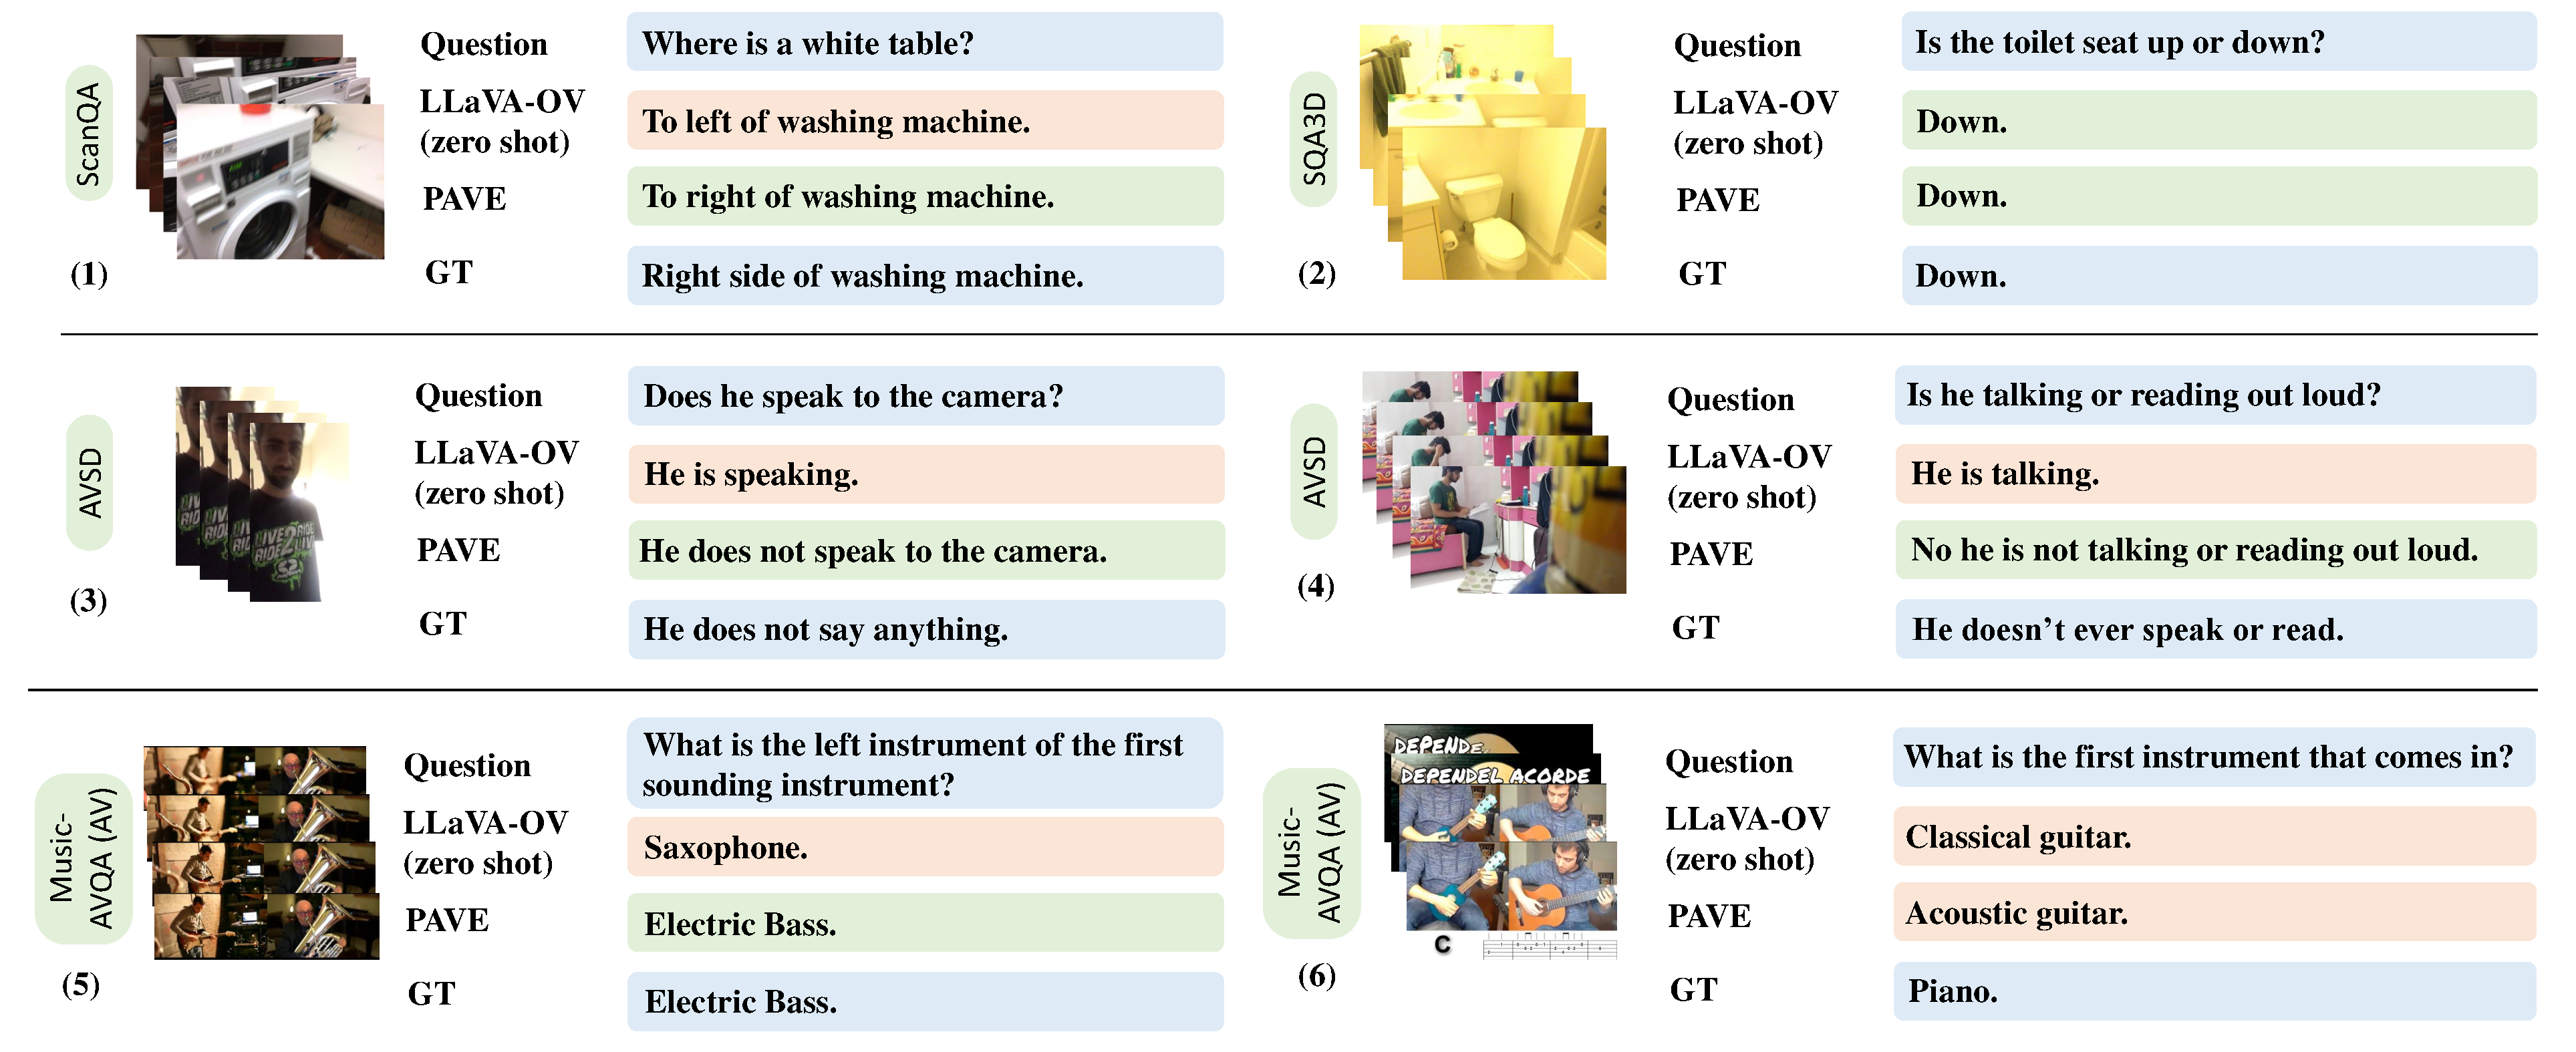
\includegraphics[width=0.92\linewidth]{figures/qa_visualization_updated2.pdf}
    \vspace{-1em}
    \caption{\textbf{Visualization of sample results}. We visualize the compare the results from our base model LLaVA-OneVision (under zero-shot inference) and PAVE across 3D QA and audio-visual QA tasks. Both succeful and failure cases are shown. 
    }
    %PAVE adapts LLaVA-OneVision to 3D QA and audio-visual tasks. The visualization provides the predictions from LLaVA-OneVision (zero-shot) and PAVE. PAVE learns to utilize 3D information and audio information for reasoning and thus improves the model performance. Specifically, in sample (6), when visual information conflicts with the audio information, the visual information will prevail given that PAVE is based on a Video LLM that is pre-trained on a visual-only dataset.}
    \label{fig:qa_visualization}
    \vspace{-0.5em}
\end{figure*}


\begin{figure*}[t!]
    \centering
    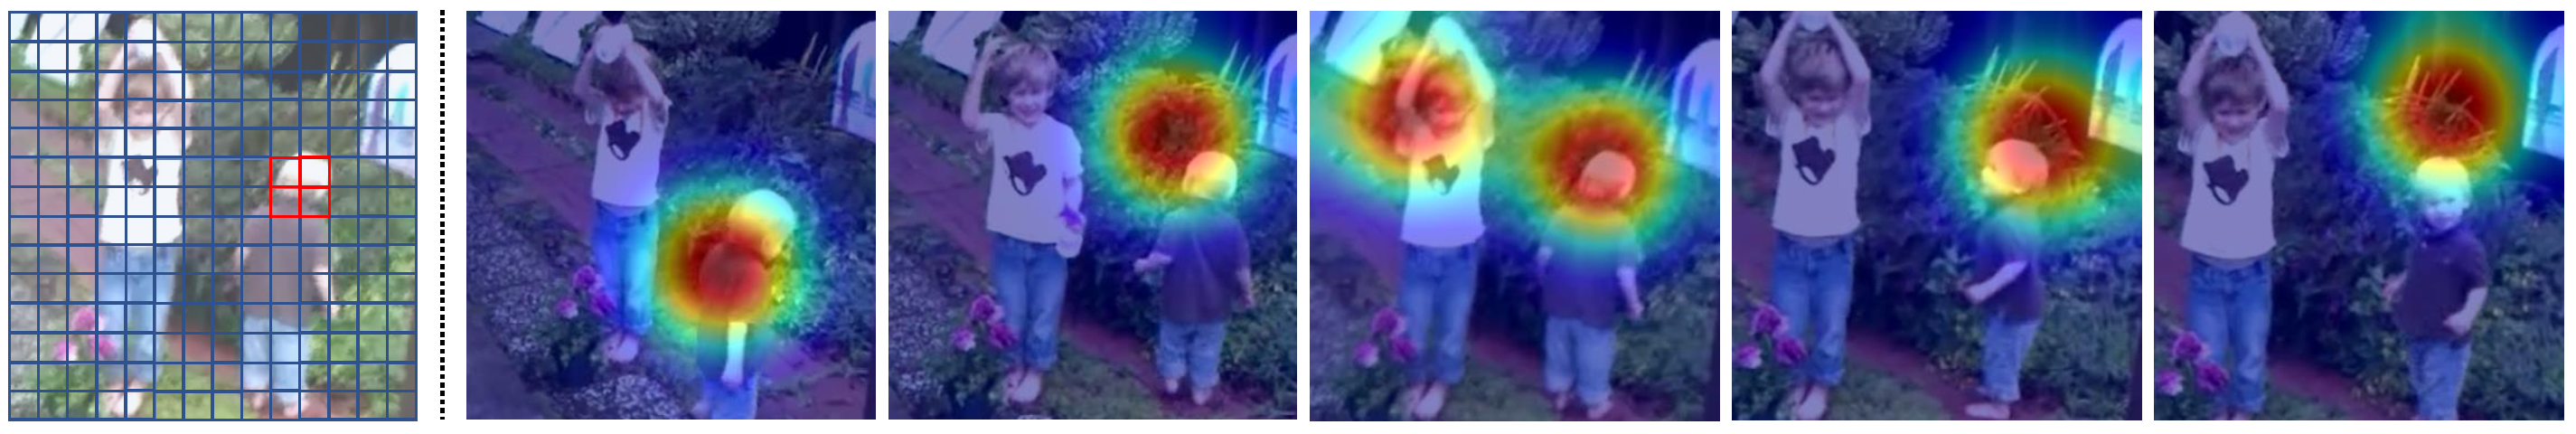
\includegraphics[width=0.90\linewidth]{figures/cross_attention_visualization.pdf}
    \vspace{-0.5em}
    \caption{\textbf{Visualization of cross-attention scores in PAVE} when injecting high frame rate videos as the side-channel. Cross-attention scores are calculated between the selected video tokens from the original low frame rate video (red cells on the left) and side-channel tokens from the high frame rate video. Scores are displayed as heatmaps over densely sampled video frames (on the right).} %This shows that cross-attention can effectively collect related information from densely sampled video frames.}
    \label{fig:cross_attention}
    \vspace{-1.5em}
\end{figure*}

\medskip
\noindent \textbf{Multi-task learning.} Moreover, we explore the potential of training multiple patches simultaneously and study the effects of such multi-task learning. We consider the setting of multiple tasks share overlapping side-channels (\eg, high-frame-rate video). In this case, multiple patches can be learned jointly, leading to potential enhancement across their corresponding side-channels.

As a first step to demonstrate this possibility, we design an experiment to integrate high frame rate video patch and audio-visual path for high frame rate audio-visual QA. Specifically, we build on the patch learned for injecting high frame rate videos (PAVE-7B model in Table~\ref{tab:general_video_understanding}), and train an additional patch for audio-visual QA on the AVSD training set. During training, the old patch is kept frozen and only the audio-visual patch is learned.  During the inference, we activate both patches, and PAVE takes input key frames (\ie low frame rate video), high frame rate video, and audio as input. Table~\ref{tab:avsd_with_dense_frames} shows that our multi-task learning leads to a notable improvement (\textit{+7.5} in CIDEr scores) on the AVSD test set, demonstrating the possibility and the benefit of training multiple patches together. We provide further discussion in Sec.\ \ref{sec:conclusion}.

%There are two distinct scenarios in multi-task joint training: 1. If individual tasks (e.g., audio-visual and 3D) do not share overlapping modalities, joint training is effectively equivalent to training each task independently. In this case, only the task-relevant patch is used for each sample. 2. When multiple tasks share overlapping modalities (e.g., high-frame-rate video) beyond raw video, multiple patches are utilized during training, leading to a more comprehensive understanding of the video and potential improvement in performance.

%We conduct additional experiments to demonstrate modality enhancement. Specifically, we use the enhanced video understanding patch (PAVE-7B model in Table~\ref{tab:general_video_understanding}) and train a new patch for audio-visual QA on the AVSD training set with the enhanced video understanding patch frozen. During the inference, we activate both patches, and PAVE takes input key frames, high framerate video, and audio as input. Table~\ref{tab:avsd_with_dense_frames} shows multi-task joint training results in a notable improvement (\textbf{+7.5}) on the AVSD test set, demonstrating the possibility and the benefit of training multiple patches together. We provide further discussion in the Appendix about leveraging multiple patches at the same time.

% Yin: The text was very redundant. DO NOT REPEAT THE TEXT IN THE PAPER.

\medskip
\noindent\textbf{Results visualization and diagnosis.} 
Finally, we visualize sample results of 3D QA and audio-visual QA in Figure~\ref{fig:qa_visualization}. An interesting failure case of PAVE, as we previously mentioned in Sec.\ \ref{section_res_audio} is shown in sample (6), where the piano is present in the audio but never appears visually in the video, creating a conflict between the auditory and visual information. In this case, PAVE produces inaccurate answers.

To further diagnose our model, we visualize cross-attention scores between video tokens and side-channel tokes in PAVE's fusion function. Figure~\ref{fig:cross_attention} shows  heatmaps of cross-attention scores when injecting high high frame rate videos as the side-channel (corresponding to results of PAVE-7B in Table~\ref{tab:general_video_understanding}). We calculate the cross-attention scores between the selected video tokens (shown in the red cells) from the original low frame rate videos, and the side-channel tokens from the high frame rate videos. The visualization shows that the peaks of the heatmap keep track of visually similar regions in densely sampled video frames. This result indicates that the fusion function in PAVE facilitates explicit alignment between video tokens and side-channel tokens, and thus allows for effectively integrating information from the side-channel.

%the heatmap has the highest response on the regions that contain a similar visual concept as the one represented by selected tokens from $\mathbf{z}^v$. 



%Figure~\ref{fig:qa_visualization} further visualizes results of 3D and audio-visual QA. 

%For 3D QA, PAVE adapts LLaVA-OneVision by incorporating additional spatial information, enabling the model to understand the relative positions of objects within the scene. 
%In the audio-video setting, PAVE enhances Video LLM's reasoning capabilities by incorporating audio input, thereby improving the model's performance and mitigating hallucination in audio-visual scenarios.
%Specifically, we visualize samples from the audio-visual split of Music-AVQA in (5) and (6). For sample (6) in Figure~\ref{fig:qa_visualization}, the piano is present in the audio but never appears visually in the video, creating a conflict between the auditory and visual information. In this case, PAVE produces inaccurate responses.
%We hypothesize that since the Video LLM that PAVE adapted is trained on visual-only data, the visual information has a higher influence than audio, which ultimately skews the prediction.


%\medskip
%\noindent\textbf{Visualization of cross-attention in PAVE.} 
%Figure~\ref{fig:cross_attention} visualizes the cross-attention map in enhanced video QA. In this setting, we use the densely sampled video frames as the side-channel information. We calculate the cross-attention activation values between the selected tokens (shown in the red cells) from the Video LLM visual encoder $\mathbf{z}^v$, and the tokens from the side-channel $\mathbf{z}^s$. The visualization indicates that the heatmap has the highest response on the regions that contain a similar visual concept as the one represented by selected tokens from $\mathbf{z}^v$. This indicates the cross-attention module captures the similarity of the visual concept between $\mathbf{z}^v$ and $\mathbf{z}^s$ and thus enables PAVE to effectively collect information from the side-channel.



%
\section{Conclusion and Discussion}
\label{sec:conclusion}

% In this paper, we consider the problem of adapting pre-trained video-LLMs to downstream tasks that feature temporal supplementary signals alongside videos. This setting covers a wide range of key challenges in video understanding, including audio-visual understanding, 3D reasoning, and video representation learning. We show that fine-tuning pre-trained video-LLMs results in competitive performance on these tasks---a finding that reconfirms the impressive reasoning capability of the latest video-LLMs. 


% Targeting at this setting, we introduce PAVE, a framework designed to adapt pre-trained video large language models (LLMs) to downstream tasks using side-channel signals. The core concept of PAVE centers on adaptation through patching, which involves introducing a small number of additional parameters and operations with minimal computational cost, all while preserving the base model architecture and pre-trained weights. PAVE effectively adapts video-LLMs for tasks such as audio-visual understanding and 3D reasoning, surpassing state-of-the-art task-specific models with less than 1\% additional parameters and FLOPs. Additionally, PAVE enhances video understanding by integrating high-frame-rate videos. We hope our work sheds light on adapting MLLMs for diverse tasks and unifying multi-modal information to support complex reasoning.


In this paper, we addressed the problem of adapting pre-trained Video LLMs to downstream tasks involving side-channel signals --- additional modalities or data types such as audio, 3D cues, high frame rate or multi-view videos.  
% 
To this end, we presented PAVE, a flexible framework that enables adaptation through patching. 
%
PAVE built on lightweight adapters (\ie, ``patches''), which adds a small number of parameters and operations ($\sim$0.1\%) to a base model without modifying its architecture or pre-trained weights.
%
We demonstrated that PAVE can effectively adapt various video LLMs across multiple tasks, often surpassing state-of-the-art task-specific models. 
%
Additionally, we showed encourage results of learning across multiple tasks with PAVE.
%
We believe that our work provides a solid step towards adapting Video LLMs for diverse tasks, and sheds light on the broader topic of multi-modal reasoning.

% Yin: The following discussion can be commented out if more space is needed.

\medskip
\noindent \textbf{Distributing and deploying tasks-specific patches.} A key strength of PAVE is that only a small patch is need for adapting a large pre-trained Video LLM to a new task. For example, for LLaVA-OneVision-7B, this patch is only $\sim$20 MB, while the model occupies $\sim$16 GB. We anticipate that this compactness makes it practical to distribute and deploy individual patches, similar to LoRA weights used in diffusion models, thereby facilitating broader adoption of Video LLMs in downstream applications.

\medskip
\noindent \textbf{Towards multi-task learning.} An exciting future research direction is the joint learning of multiple patches across tasks. While we have demonstrated the feasibility of stage-wise multi-task learning, future work should aim to handle multi-task joint training and explore methods for combining individual patches to enable flexible task composition. 



\begin{comment}
To adapt to a new task, PAVE only needs to issue a small patch (\eg 20 MB) with the LoRA weights on top of the vanilla video-LLM, which needs around 16 GB to store its parameters. It adds negligible parameters and operations with minimal computational cost while preserving the base model architecture and pre-trained weights. 

we present PAVE, a flexible framework for adapting pre-trained Video LLMs to downstream tasks with side-channel signals, such as audio, 3D cues, or multi-view videos.
PAVE introduces lightweight adapters, referred to as ``patches,'' which adds a small number of parameters and operations to a base model without modifying its architecture or pre-trained weights. In doing so, PAVE can effectively adapt the pre-trained base model to support diverse downstream tasks, including audio-visual question answering, 3D reasoning, multi-view video recognition, and high frame rate video understanding. Across these tasks, PAVE significant enhances the performance of the base model, surpassing state-of-the-art task-specific models while incurring a minor cost of $\sim$0.1\% additional FLOPs and parameters. Further, PAVE supports multi-task learning and generalizes well across different Video LLMs.

PAVE effectively adapts video-LLMs for tasks such as audio-visual understanding, 3D reasoning, and multi-view video understanding, surpassing state-of-the-art task-specific models. 

that feature temporal supplementary signals alongside videos. 
% This setting covers various key challenges in video understanding, including audio-visual understanding, 3D reasoning, and video representation learning. 
Targeting this setting, we introduced PAVE, a framework that leverages a patching mechanism to adapt existing video-LLMs with additional side-channel information. To adapt to a new task, PAVE only needs to issue a small patch (\eg 20 MB) with the LoRA weights on top of the vanilla video-LLM, which needs around 16 GB to store its parameters. It adds negligible parameters and operations with minimal computational cost while preserving the base model architecture and pre-trained weights. 
PAVE effectively adapts video-LLMs for tasks such as audio-visual understanding, 3D reasoning, and multi-view video understanding, surpassing state-of-the-art task-specific models. 
% Our method thus put a question mark on the necessity of task-specific pre-training. 
Additionally, PAVE can enhance video understanding by integrating high-frame-rate videos. 
We hope our work sheds light on adapting MLLMs for diverse tasks and unifying multi-modal information to support complex reasoning.
\end{comment}

% Yin: This acknowledgment can stay in page 9. 
\medskip
\noindent \textbf{Acknowledgment}: This work was partially supported by National Science Foundation under Grant No.\ CNS 2333491, by the Army Research Lab under contract number W911NF-2020221, and by a contract from General Motors. 
{
    \small
    \bibliographystyle{ieeenat_fullname}
    \bibliography{main}
}

% WARNING: do not forget to delete the supplementary pages from your submission 
\clearpage
%\clearpage
% \FloatBarrier
\appendix
In this supplement, we (1) show additional experiment results on small Video LLM and multiple-view video understanding (Section~\ref{experiment}); (2) describe additional implementation details (Section~\ref{implementation}); (3) include additional visualization of the question-answering results (Section~\ref{visualization}).
% and (4) provide further discussion of setting of using multiple patches and potential future work (Section~\ref{discussion}). 
%We hope that this document will complement our main paper. 

% For sections, figures, tables, and equations, we use numbers (e.g., Sec. 1) to refer to the main paper and capital letters (e.g., Sec. A) to refer to this supplement.
\begin{table*}[t]  
\centering  
\scalebox{0.77}{
\begin{tabular}{lc|c|cccc|c|c}  
\toprule
       \multirow{2}{*}{Method}      & AVSD~\cite{alamri2019audiovisualsceneawaredialog}  &AVQA~\cite{yang2022avqa}&\multicolumn{4}{c|}{MUSIC-AVQA~\cite{Li2022Learning}}  & \multirow{2}{*}{TFLOPs} & \multirow{2}{*}{Total / Trainable Params} \\
                                    & CIDEr                                              & Acc. &Audio Acc. & Visual Acc. & Audio-Visual Acc.  & Overall Acc. & & \\
    \midrule
    \multicolumn{3}{l}{\it \small\textbf{Zero-shot LMMs} } \\
     %CAT-7B ~\cite{ye2024catenhancingmultimodallarge}             & 79.0 & -  & -  & -    & -    & 48.6 & -      & - \\
     LLaVA-OV-0.5B~\cite{li2024llava}                             & 65.1 & 77.4 & \textcolor{gray}{60.0} & 57.1 & 48.5 & 52.8 & 8.01 & 0.9B~/~-\\
     LLaVA-OV-7B~\cite{li2024llava}                               & 70.6 & 85.6 & \textcolor{gray}{68.8} & 70.6 & 52.8 & 60.4 & 98.53 & 8.2B~/~-\\
     \midrule
     \multicolumn{3}{l}{\it \small\textbf{Task-specific models} } \\     
     %MTN~\cite{Le_2019}                                           & 98.5  & -  & - & - & -  &  - &-  & -\\
     %COST~\cite{pham2022videodialogconversationobjects}           & 108.5 & -  & - & - & -  &  - &-  & - \\
     %VALOR~\cite{chen2023valorvisionaudiolanguageomniperceptionpretraining} & -  & - & - & -  & -&  78.9 & - & - \\
     %VAST~\cite{chen2023vast} & -  & - & - & -  & -&  80.7 & - & - \\
     %PSTP-Net~\cite{li2023progressive} & -  & 90.2 & - & -  & -&  - & - & - \\
     %CAT-7B-FT ~\cite{ye2024catenhancingmultimodallarge}          & - & 92.0 & \textcolor{gray}{\textbf{84.9}} & 86.1 & \textbf{83.2} &    \textbf{84.3} & -  & - \\ %0.6492%
     LLaVA-OV-0.5B-FT                                             & 117.6  & 86.4 & \textcolor{gray}{69.6} & 76.3 & 62.8 &  67.6  & 8.01 & 0.9B~/~35.2M \\
     LLaVA-OV-7B-FT                                               & 124.9  & 90.8 & \textcolor{gray}{75.4} & 89.3 & 72.3 &  77.4  & 98.53 & 8.2B~/~161.5M \\
     \midrule
     
     PAVE-0.5B (w/ audio)                                          & 134.5 &  90.4  & \textcolor{gray}{77.3} & 89.8  & 74.1 & 78.8 & 8.08 & 0.9B~/~41.4M   \\
     PAVE-7B   (w/ audio)                                          & 152.9 & 93.8 & \textcolor{gray}{79.7} & 93.0 & 78.0 &  82.3 & 98.63 & 8.2B~/~170.5M \\ \bottomrule

\end{tabular}
}


% \vspace{-1mm}
\caption{Additional result of PAVE on the audio-visual understanding tasks with audio as additional information. 
\vspace{-1mm}
}  
\label{tab:video_audio_understanding_appendix}  
\end{table*}  

\begin{table*}[t]  
\centering  
\scalebox{0.8}{
\begin{tabular}{lccccc|c|c|c}  
\toprule
\multirow{2}{*}{Method}                                          & \multicolumn{5}{c|}{ScanQA~\cite{azuma_2022_CVPR}} & SQA3D\cite{ma2022sqa3d} & \multirow{2}{*}{TFLOPs} & \multirow{2}{*}{Total / Trainable Params}\\
                                                                 & C     & B-4 & M     & R    & EM@1 & EM@1     &&            \\ 
    \midrule
    \multicolumn{6}{l}{\it \small\textbf{Zero-shot LMMs}} \\
     %VideoChat2-7B~\cite{li2024mvbenchcomprehensivemultimodalvideo} & 49.2  & 9.6 & 9.5   & 28.2 & 19.2 & 37.3 & - & - \\
     LLaVA-OV-0.5B~\cite{li2024llava}                            & 17.2  & 1.2 & 13.7  & 18.4 & 0.2 \textcolor{gray}{(28.0)} & 0.8 \textcolor{gray}{(43.0)} & 8.01 & 0.9B~/- \\
     LLaVA-OV-7B~\cite{li2024llava}                              & 91.0  & 5.3 &  18.2 & 45.9 & 26.7 \textcolor{gray}{(44.3)} & 8.3 \textcolor{gray}{(50.7)} &98.53 & 8.2B / - \\
    \midrule
    \multicolumn{6}{l}{\it \small\textbf{Task-specific models}} \\
     %Scene-LLM-7B~\cite{fu2024scenellmextendinglanguagemodel}       &  80.0 & 12.0 & 16.6 & 40.0 & 27.2 & 54.2 & - & - \\
     %LLaVA-3D-7B~\cite{zhu2024llava3dsimpleeffectivepathway}        &  91.7  & 14.5 & \textbf{20.7} & \textbf{50.1} & 27.0 \textcolor{gray}{(45.0)} & 55.6 \textcolor{gray}{(57.6)} & - & - \\%14.35%
      % LLaVA-3D (re-eval)                                         &  83.8  & 10.8 & 16.7 & 42.6 & 25.7 \textcolor{gray}{(45.1)}            &  & - & - \\
      LLaVA-OV-0.5B-FT  & 70.5 & 6.5 & 14.3 & 36.9 & 20.5 \textcolor{gray}{(36.3)}  & 44.1 \textcolor{gray}{(45.7)} & 8.01 & 0.9B~/~35.2M\\
      LLaVA-OV-7B-FT    & 95.1 & 13.5 & 19.1 & 47.4 & 27.4 \textcolor{gray}{(46.3)} & 55.8 \textcolor{gray}{(58.1)} & 98.53 & 8.2B / 161.5M \\
    \midrule
     PAVE-0.5B (w/ 3D info)                                       & 84.2 & 13.1 & 17.0 & 42.1 & 23.1 \textcolor{gray}{(40.0)}&  51.1 \textcolor{gray}{(52.8)} & 8.13 & 0.9B~/~41.4M\\
     PAVE-7B   (w/ 3D info)                                       & 103.4 & 16.0 & 19.9 & 49.0 & 29.1 \textcolor{gray}{(48.5)} & 59.0 \textcolor{gray}{(61.4)} & 98.68 & 8.2B / 170.5M\\ \bottomrule
     

\end{tabular}
}
% \vspace{-1mm}
\caption{Additional result of PAVE on the 3DQA tasks with 3D information as additional information.
}  
\vspace{-1mm}
\label{tab:3d_qa_understanding_appendix}  
\end{table*}  



\begin{table*}[t]  
\centering  
\scalebox{0.72}{
\begin{tabular}{l|ccccc|c|c}  
\toprule
% \multirow{2}{*}{Method}   & \multicolumn{4}{c|}{VideoMME~\cite{fu2024video}} & \multicolumn{4}{c|}{MVBench~\cite{li2023mvbench}} & \multirow{2}{*}{MLVU~\cite{zhou2025mlvubenchmarkingmultitasklong}}  & \multirow{2}{*}{FLOPs(TB)} & \multirow{2}{*}{Total / Trainable Params}  \\
     Method                               & ActivtityNet-QA & EgoSchema & NextQA & PerceptionTest & VideoMME (w-subs) & FLOPs (TB) & Total / Trainable Params \\ 
    \midrule
     LLaVA-OV-0.5B~\cite{li2024llava}     & 50.5            & 26.8      & 57.2   & 49.2            & 43.5 & 8.01 & 0.9B~/~- \\
     LLaVA-OV-7B~\cite{li2024llava}       & 56.6            & 60.1      & 79.4   & 57.1            & 61.5 & 98.53 & 8.2B~/~- \\
     \midrule
     PAVE-0.5B (w/ video feature)         & 50.6 & 27.1  &    56.1 & 48.8 & 48.6 & 8.08  & 0.9B~/~41.4M  \\
     PAVE-7B   (w/ video feature)         & 57.1 & 57.4  &    79.6 & 56.0 & 62.9 & 98.63 & 8.2B~/~170.5M \\ \bottomrule

\end{tabular}
}
% \vspace{-1mm}
\caption{Result of PAVE on the additional benchmarks in enhanced video understanding setting. PAVE uses densely sampled video frames as additional information. 
\vspace{-1mm}
}  
\label{tab:general_video_understanding_appendix}  
\end{table*}  




\section{Additional Experiment Results} \label{experiment}
% \subsection{The Experiments with Small Language Model.}
\subsection{Results with small Video LLM} 

We now present additional experiment results of PAVE with LLaVA-OneVision 0.5B models for audio-visual QA and 3D QA. 
Table~\ref{tab:video_audio_understanding_appendix} and Table~\ref{tab:3d_qa_understanding_appendix} show the results. PAVE consistently improves the 0.5B and 7B Video LLM's performance by a large margin across both settings. 
% Specifically, we observed a significant performance gap between LLaVA-OV-FT and PAVE. 
This indicates that PAVE effectively leverages additional information when adapting pre-trained Video LLMs into new settings. 

\subsection{Results on Enhanced Video Understanding} 

We present PAVE's result on additional benchmarks in the enhanced video understanding setting. 
% These results were omitted from the main paper due to space limit.
Table~\ref{tab:general_video_understanding_appendix} shows PAVE's results in the enhanced video understanding setting with additional benchmarks. PAVE demonstrates a substantial performance gain on VideoMME (w-subtitles). However, we observe only marginal or no improvement on ActivityNet-QA, EgoSchema, NextQA, and PerceptionTest. We hypothesize that this discrepancy may be due to: (1) domain shift—our training data primarily consists of third-person view videos, which may lead to a performance drop in EgoSchema, and (2) the nature of the benchmark questions, which may not require densely temporal information for reasoning.





\begin{table}[t]  
\centering
% \vspace{-1em}
\resizebox{0.98\linewidth}{!}{
\begin{tabular}{lccc}  
\toprule
       Model                    & Acc. & FLOPs (TB) &  Total / Trainable Params \\
     \midrule
     \multicolumn{4}{l}{\it \small\textbf{Zero-shot LMMs}} \\
     LLaVA-OV-0.5B    &  23.6   & 8.01  & 0.9B~/ -   \\
     LLaVA-OV-7B   &  23.6    & 98.53  & -    \\
     \midrule
     \multicolumn{4}{l}{\it \small\textbf{Task-specific models}} \\
     LLaVA-OV-0.5B-FT             & 28.2     & 8.01  & 0.9B~/~35.2M  \\
     LLaVA-OV-7B-FT             & 29.8     & 98.53  & 8.2B / 161.5M  \\
     TimeSFormer (Ego+Exo)* ~\cite{grauman2024ego}      & 43.7    & -  &   -  \\
     % TimeSFormer (Ego)        & 47.2  & -  &   -  \\
     % TimeSFormer (Ego+Exo)* ~\cite{grauman2024ego}      & 43.7    & -  &   -  \\
     % CAT-7B-FT                  & -   & 92.0 & -  &   -  \\
     \midrule
     PAVE-0.5B                & 32.4           & 8.15 & 0.9B~/~41.4M \\ 
     PAVE-7B                  & 44.2  & 98.70 & 8.2B / 170.5M \\ 
     % PAVE-AVQA                & -   & \textbf{93.8} & 8.00 & 8.2B / 170.4M\\ 
     \bottomrule

\end{tabular}
}
\vspace{-2mm}
%\caption{Result of multi-view video recognition on Ego-Exo4D
\caption{Performance of PAVE on multi-view video understanding with Ego-Exo4D Demonstrator Proficiency benchmark. LLaVA-OV-7B-FT refers to directly fine-tuning the LLaVA-OneVision on the training set. Our model achieves state-of-the-art performance by only adding a small amount of parameters and FLOPs. * means this baseline may use more training data than PAVE because some of the videos are unavailable to us.} 
\label{tab:ego_exo_videos_appendix}  
\end{table}


\subsection{Results on Multi-view Video Understanding} \label{section_res_multi_view_video}
\noindent\textbf{Motivation and task set up.}
Understanding human activity from video is crucial in many real-world applications, such as augmented reality and robotic learning. Based on the perspective, videos can be broadly classified into ego-centric and exo-centric views. Ego-centric videos capture first-person interactions, focusing on close-up hand-object interactions, while exo-centric videos provide a third-person perspective, recording full-body postures and the surrounding environment. Both perspectives are essential for comprehensive human action understanding. 
Different from the audio-visual QA and 3D QA, where the side-channel information comes from other modalities, in this context, PAVE regards exo-centric videos as side-channel information and integrates it with ego-centric video to adapt the Video LLMs for multi-view video understanding.

\medskip
\noindent\textbf{Training data.} 
We use the training set from the Ego-Exo4D demonstrator proficiency estimation benchmark~\cite{grauman2024ego} as our training data, which consists of 1,904 question-answer pairs. Each pair is associated with one ego-centric video and four exo-centric videos. The task requires the model to classify human action proficiency into one of four categories: Novice, Early Expert, Intermediate Expert, or Late Expert, based on both ego- and exo-centric videos. However, only 1,656 question-answer pairs include the corresponding videos, as the videos for the remaining pairs could not be downloaded due to privacy issues.


\medskip
\noindent\textbf{Implementation details.}
Considering the exo- and ego-centric videos are synchronized along the temporal axis, we sample 32 frames for each of the exo-centric videos. To keep the encoding procedure consistent between the ego- and exo-video, we use the same preprocessing of the LLaVA-OneVision to reshape and crop the video frames. We use SigLIP~\cite{zhai2023sigmoidlosslanguageimage} as the visual encoder and it encodes and downsamples each frame into 196 tokens. We pre-extract the exo-video feature tokens offline to accelerate the training. 
We build PAVE on top of LLaVA-OneVision~\cite{li2024llava} and train the model for 2 epochs.


\medskip
\noindent\textbf{Evaluation benchmark.} 
We use the validation set of the Ego-Exo4D~\cite{grauman2024ego} demonstrator proficiency estimation benchmark for evaluation and report accuracy as the metric. It contains 466 questions and each of the questions is paired with 1 ego-centric video and 4 exo-centric videos.
% what metriec we use 
% how many question we have 
% what is the qiestion look like 

\medskip
\noindent\textbf{Baselines.}
% baseline from the egoexo
% baseline by fineting the model
We use the TimeSFormer (Ego+Exo) from Ego-Exo4D~\cite{grauman2024ego} as our baseline. We also include a baseline that directly fine-tunes the LLaVA-OneVision with LoRA on the training set without using the exo-centric videos, denoted as LLaVA-OV-7B-FT. This baseline allows us to assess whether PAVE can effectively utilize supplementary information.

\medskip
\noindent\textbf{Results.} Table~\ref{tab:ego_exo_videos_appendix} shows the results of PAVE. Compared with the LLaVA-OV-7B-FT, PAVE-7B achieves about 14.4\% improvement by adding only 9M parameters and 0.17 TFLOPs during inference. This big improvement indicates that the exo-centric videos provide crucial additional information for human action understanding.
Moreover, PAVE achieves state-of-the-art performance on the demonstrator proficiency estimation benchmark, substantiating that  PAVE can adapt a pre-trained Video LLM to an unseen setting by leveraging supplementary information. 

% \begin{table}[h!]  
% \centering
% % \vspace{-1em}
% \resizebox{0.98\linewidth}{!}{
% \begin{tabular}{lccc}  
% \toprule
%        Model                    & Acc. & FLOPs (TB) &  Total / Trainable Params \\
%      \midrule
%      LLaVA-OV-7B (Zero-shot)    &  23.6    & 98.53  & -    \\
%      LLaVA-OV-7B-FT             & 29.8     & 98.53  & 8.2B / 161.5M  \\
%      % TimeSFormer (Ego)        & 47.2  & -  &   -  \\
%      TimeSFormer (Ego+Exo)* ~\cite{grauman2024ego}      & 43.7    & -  &   -  \\
%      % CAT-7B-FT                  & -   & 92.0 & -  &   -  \\
%      \midrule
%      PAVE-7B (w/ Exo-videos)             & \textbf{44.2}  & 98.70 & 8.2B / 170.5M \\ 
%      % PAVE-AVQA                & -   & \textbf{93.8} & 8.00 & 8.2B / 170.4M\\ 
%      \bottomrule

% \end{tabular}
% }
% \vspace{-2mm}
% %\caption{Result of multi-view video recognition on Ego-Exo4D
% \caption{Performance of PAVE on multi-view video understanding with Ego-Exo4D Demonstrator Proficiency benchmark. LLaVA-OV-7B-FT refers to directly fine-tuning the LLaVA-OneVision on the training set. Our model achieves state-of-the-art performance by only adding a small amount of parameters and FLOPs. * means this baseline may use more training data than PAVE because some of the videos are unavailable to us.} 
% \label{tab:ego_exo_videos}  
% \end{table}


\section{Implementation and Experiment Details} \label{implementation}
We first describe the general implementation detail of the PAVE in Section~\ref{pave_inple}. Then, we describe the experiment details for 3 settings considered in the main paper, including audio-visual QA (Section~\ref{avqa}), 3DQA (Section~\ref{3dqa}), and enhancing video QA (Section~\ref{enhanced_video_qa}). We also demonstrate how we calculate the Flops for the model in Section~\ref{flops_calc}.

\subsection{Implementation Detail of PAVE} \label{pave_inple}


Inside the temporal-aligned cross-attention layer, we add rotary position embedding to the query and key tokens. Specifically, we apply different rotary positional embedding according to the layout of side-channel tokens $\mathbf{z}^s$. We mainly consider two types of $\mathbf{z}^s$: (a) $\{\mathbf{z}^s\}$ includes both spatial and temporal dimensions, such as tokens from video backbones or from a 3D backbone; and (b) $\{\mathbf{z}^s\}$ only contains temporal dimension, such as audio tokens. For the first case, we will add 3D rotary positional embedding (along the temporal, height, and width dimensions). For the second case, we will only add rotary positional embedding along the temporal axis. After cross-attention, we use a two-layer MLP, followed by a layer norm. 
After the PAVE layers, we add another two-layer MLP, followed by a layer norm, as the adapter. We initialize the $\gamma$ in the layer norm to zero. 
% For all experiments, we use a learning rate of 2e-5 and a batch size of 32 to adapt the pre-trained Video LLM.




%%%%%%%%%%%%%%%%%%%%%%%%%%%%%%%%% AVQA
% all other things including some of the implementation details.




\subsection{Audio-Visual QA}\label{avqa}
In this setting, the input of the PAVE has two parts: (1) the visual tokens $\mathbf{z}^v$ from the Video LLM's visual encoder, and (2) the audio tokens $\mathbf{z}^s$ from a side-channel signal encoder.

\medskip
\noindent \textbf{Visual Encoder.} For $\mathbf{z}^v$, we follow the default setting used in LLaVA-OneVision~\cite{li2024llava}. We uniformly sample 32 frames from the video and use the same preprocessing of the LLaVA-OneVision to reshape and crop the video frames. We use SigLIP~\cite{zhai2023sigmoidlosslanguageimage} as the visual encoder and it encodes and downsamples each frame into 196 tokens. 


\medskip
\noindent \textbf{Side-Channel Signal Encoder.}
For $\mathbf{z}^s$, we follow the pre-processing step of ImageBind~\cite{girdhar2023imagebind}, which resamples the audio at 16KHz. 
% In order to fit into the design of the Audio Spectrogram Transformer~\cite{gong2021astaudiospectrogramtransformer}, we split the audio tokens along the temporal axis into multiple groups with each group containing 1024 tokens. We later concatenate the encoded features of all groups along the temporal axis. Audio Spectrogram Transformer will down-sample the temporal dimension by 16 and generate about 6 tokens per second with token dimension 768. 
We segment the audio into overlapping 2-second clips with a 1-second stride and encode each clip using the audio encoder of ImageBind. This process generates a 1024-dimensional audio token for every 1 second of the audio signal.
Since we do not fine-tune the audio encoder, we extract the audio feature tokens offline in order to accelerate the training.

\medskip
\noindent \textbf{Network Architecture.} For the PAVE design, we use 2 cross-attention layers with hidden dimension 512 and have 4 attention heads. 
% After the cross-attention, we add 2 layers of MLP and a layer normalization layer, in which $\gamma$ is initialized as 0 at the beginning of the training. 
For LoRA layers in the LLM, we use LoRA$\_r$ = 64 and LoRA$\_\alpha$ = 16. 

\medskip
\noindent \textbf{Training Details.}
For training, we use AdamW~\cite{loshchilov2019decoupledweightdecayregularization} optimizer with a linear warmup using the first 3\% of iterations. We use the cosine annealing learning rate during the training. We set the base learning rate as 2e-5 and the batch size as 32. All the experiments are run on 2 A100 80G GPUs. 

\medskip
\noindent\textbf{Training data.} We choose the open-end QA dataset AVSD~\cite{alamri2019audiovisualsceneawaredialog}, and closed-end QA dataset AVQA~\cite{yang2022avqa} and Music-AVQA~\cite{Li2022Learning} as training dataset. AVSD contains 79k question-answer pairs across 7,985 videos with each paired 10 questions. AVQA has 40k question-answer pairs coupled with 40k Videos. Music-AVQA consists of 32k question-answer pairs and 9277 videos.

\medskip
\noindent\textbf{Evaluation benchmark.} We follow the protocol in previous works~\cite{ye2024catenhancingmultimodallarge, pham2022videodialogconversationobjects} to evaluate PAVE. For AVSD, we use the AVSD@DSTC7 test split and report CIDEr score as the metric. This benchmark consists of 1,000 audio-visual questions.
We use COCO API~\cite{lin2015microsoftcococommonobjects} to calculate the CIDEr score between the model predictions and the ground truth answers. 
For AVQA, we evaluate PAVE on the eval split and report the accuracy as the metric. This benchmark contains 17k questions that require reasoning based on audio and visual information.
For Music-AVQA, we evaluate PAVE on the test split and report the accuracy as the metric. This benchmark contains 9185 questions, which can be categorized into visual, audio, and audio-visual questions.
% Additionally, we calculate the model inference FLOPs at the prefilling stage using LLM-Viewer~\cite{yuan2024llm}.






%%%%%%%%%%%%%%%%%%%%%%%%%%%%%%%%%%%% 3d QA

\subsection{3DQA} \label{3dqa}
In this setting, the input of the PAVE consists of two parts: (1) the visual tokens $\mathbf{z}^v$ from the Video LLM's visual encoder, and (2) the 3D tokens $\mathbf{z}^s$ from a side-channel signal encoder.

\medskip
\noindent \textbf{Visual Encoder.} For $\mathbf{z}^v$, we use the same setting as the one in Section~\ref{avqa}. 

\medskip
\noindent \textbf{Side-Channel Signal Encoder.} For encoding the side-channels information into $\mathbf{z}^s$, we utilize the 3D encoder which contains two parts 1. a visual encoder which encodes the RGB frames into visual feature tokens. 2. a spatial embedding that adds the encoded 3D information on the visual feature tokens. We uniformly extract 32 RGB-D frames from the scan and use ViT~\cite{dosovitskiy2021imageworth16x16words} to extract the visual features from the RGB frames. We then add spatial embeddings to visual features following the LLaVA-3D~\cite{zhu2024llava3dsimpleeffectivepathway} by making use of the depth information and the camera pose. It generates 576 tokens for each frame, with a token dimension of 1024. We pre-extract the 3D feature to accelerate the training.


\medskip
\noindent \textbf{Network Architecture and Training Details.} For the PAVE design and the training configuration, we use the same hyper-parameters used in Section~\ref{avqa}.

% \noindent\textbf{3DQA Implementation details.}
% To encode 3D information, we follow the LLaVA-3D~\cite{zhu2024llava3dsimpleeffectivepathway} that adds spatial embeddings to the visual tokens generated by ViT~\cite{dosovitskiy2021imageworth16x16words}. Since the videos are relatively short in the 3D setting, we evenly sample 32 RGB-D frames from the scanning videos. We send the RGB-D frame with the camera pose into the ViT backbone and generate 18432 tokens per scan. 
% We build PAVE on top of LLaVA-OneVision\cite{li2024llava}. We train the PAVE with ScanQA / SQA3D training set when evaluating PAVE performance on ScanQA / SQA3D, respectively. For ScanQA experiments, we train PAVE for one epoch on its training set, whereas for SQA3D, we train PAVE for two epochs.

\medskip
\noindent\textbf{Training data.} For 3D QA tasks, we consider ScanQA~\cite{azuma_2022_CVPR} and SQA3D~\cite{ma2022sqa3d}. ScanQA and SQA3D contain 25K and 26K training question-answer pairs, respectively. They share the same scanning data set which contains 562 3D scanning from ScanNet~\cite{dai2017scannet}. 


\medskip
\noindent\textbf{Evaluation benchmark.} We report our model performance on the ScanQA validation set, which contains 4,675 questions covering both object position reasoning and object recognition, and the SQA3D test set with 3519 questions, which consists of 5 different types of questions.
Following previous work~\cite{zhu2024llava3dsimpleeffectivepathway}, we report the CIDEr (C), BLEU-4 (B-4), METEOR (M), ROUGE(R), and top-1 Exact Match (EM@1) metrics on ScanQA and report EM@1 on SQA3D. We use the evaluation pipeline set up by LLaVA-3D to evaluate our model on ScanQA and SQA3D. 
% We also calculate the model inference FLOPs at the prefilling stage using LLM-Viewer~\cite{yuan2024llm}.




%%%%%%%%%%%%%%%%%%%%%%%%%%% multi view %%%%%%%%%%%%%%%%%%

% \subsection{Multi-view Video Understanding} \label{multi_view}
% In this setting, the input of the PAVE consists of two parts: (1) the ego-centric visual tokens $\mathbf{z}^v$ from the Video LLM's visual encoder which encodes the ego-centric video, and (2) the exo-centric the visual tokens $\mathbf{z}^s$ from the Side-Channel signal encoder which encodes the exo-centric videos.


% \medskip
% \noindent \textbf{Visual Encoder.} For $\mathbf{z}^v$, we use the same setting as the one in Section~\ref{avqa}. 

% \medskip
% \noindent \textbf{Side-Channel Signal Encoder.} Considering the exo- and ego-centric videos are synchronized along the temporal axis, we sample 32 frames for each of the exo-centric videos. To keep the encoding procedure consistent between the ego- and exo-video, we use the same preprocessing of the LLaVA-OneVision to reshape and crop the video frames. We use SigLIP~\cite{zhai2023sigmoidlosslanguageimage} as the visual encoder and it encodes and downsamples each frame into 196 tokens. We pre-extract the exo-video feature tokens offline in order to accelerate the training.

% \medskip
% \noindent \textbf{Network Architecture and Training Details.} For the PAVE design and the training configuration, we use the same hyper-parameters used in Section~\ref{avqa}.



%%%%%%%%%%%%%%%%%%% Enhanced Video QA

\subsection{Enhancing Video QA} \label{enhanced_video_qa}
In this setting, the input of the PAVE has two parts: (1) the visual tokens from the Video LLM's visual encoder $\mathbf{z}^v$, extracted at sparsely sample video key frames, and (2) the side-channel visual tokens $\mathbf{z}^s$, derived from a high frame rate video.

\medskip
\noindent \textbf{Visual Encoder.} For $\mathbf{z}^v$, we use the same setting as the one in Section~\ref{avqa}.  
%For $\mathbf{z}^v$, we use the same setting as the one in Section~\ref{avqa}. 

\medskip
\noindent \textbf{Side-Channel Signal Encoder.} In this case, the side-channel signals $\mathbf{z}^s$ are high frame rate videos. We sample the video frames at the frame rate of 2fps and use the default pre-processing step of the LanguageBind to reshape and crop the video frames. To leverage LanguageBind~\cite{zhu2023languagebind} to encode the high-frame-rate video frames, we split the video frames along the temporal axis into multiple non-overlap groups with each group containing 8 frames. We later concatenate the encoded features of all groups along the temporal axis. To reduce the overhead of the PAVE, inspired by the Slow-Fast~\cite{feichtenhofer2019slowfastnetworksvideorecognition}, we downsample the spatial resolution of the video feature of each video frame from 16 $\times$ 16 to 2 $\times$ 2. We do not utilize the classification tokens from the output of the LanguageBind. Since we do not fine-tune LanguageBind's video encoder, we pre-extract the video features in order to speed up the training.

\medskip
\noindent \textbf{Network Architecture and Training Details.} For the PAVE design and the training configuration, we use the same hyper-parameters used in Section~\ref{avqa}.

% and train PAVE for 1 epoch on the ScanQA training set and 2 epochs on SQA3D training set. We train PAVE on ScanQA / SQA3D training set when we evaluate PAVE performance on ScanQA / SQA3D, respectively.

% \noindent\textbf{Enhanced QA Implementation details.} We choose the LanguageBind~\cite{zhu2023languagebind} as the video backbone which can produce text-aligned video features. We sample the video features at 2 fps. Motivated by Slow-Fast~\cite{feichtenhofer2019slowfastnetworksvideorecognition}, we downsample the spatial resolution to $2 \times 2$ and treat the additional video features as a fast stream. 
% These new video features are densely sampled along the temporal axis, yet with low spatial resolution. 
% We build PAVE on top of LLaVA-OneVision~\cite{li2024llava} and train the model for 1 epoch on the subset we created.

\medskip
\noindent\textbf{Training data.} We create a subset from LLaVA-Video-178K \cite{zhang2024videoinstructiontuningsynthetic} by first sampling all videos longer than 1 minute and then randomly choosing 2 question-answer pairs for each video. This process creates a training set that contains 57K videos and 114K question-and-answer pairs. 


\medskip
\noindent\textbf{Evaluation benchmark.} We use VideoMME~\cite{fu2024video}, MVBench~\cite{li2023mvbench}, and MLVU~\cite{zhou2025mlvubenchmarkingmultitasklong} as evaluation benchmarks. VideoMME and MVBench are both comprehensive video benchmarks and cover different types of subtasks, while MLVU focuses on long video understanding.
VideoMME includes 6 key domains and 30 sub-classes. It contains 900 videos, ranging from less than one minute to nearly one hour. There are 2,700 questions with each accompanied by four options. %, using accuracy as the evaluation metric.
MVBench includes 20 different sub-tasks, such as object shuffling and fine-grained pose estimation, which require detailed temporal information. In total, it has about 4000 questions and 3900 videos. % It uses accuracy as the evaluation metric. 
MLVU contains 2175 questions and 1337 long videos.
All benchmarks adopt accuracy as the performance metric.
% We use the lmms-eval\cite{zhang2024lmmsevalrealitycheckevaluation} system to evaluate our model on these two benchmarks.
% Besides, we also calculate the inference FLOPs at the prefilling stage using LLM-Viewer~\cite{yuan2024llm}.


\subsection{The Calculation of Inference FLOPs.} \label{flops_calc}
We now describe how the floating-point operations (FLOPs) are reported in our experiments.
%On tables in main paper we present the Flops of the model at prefilling stage during inference time. 
% FLOPs of Large Language Model (LLM) dominates the total FLOPs of the video LLM. For example, the LLM in LLaVA-OV-7B has 97.8TB FLOPS, its visual encoder has only 1.8TB FLOPs. Similarly, the audio / 3D encoder in our audio-visual / 3D QA has about 70.4GB / 1.5TB FLOPs, respectively. 
Since the visual-encoder and the side-channel information encoder are replaceable modules in PAVE settings (i.e. we can use encoder with different scales at different settings.), we only consider the FLOPs of PAVE and LLM, provided by the LLM-Viewer~\cite{yuan2024llm}. During the FLOPs calculation of LLM, we consider 6272 visual tokens, and following the previous work~\cite{shang2024llavaprumergeadaptivetokenreduction}, we add 40 additional tokens for the text. We then calculate and add the FLOPs of PAVE. 

%To account for the additional FLOPs introduced by the PAVE, we calculate the FLOPs of the PAVE for each case and add it onto the FLOPs of the Video LLM. 
%



The FLOPs of PAVE is calculated as follows. The input of the PAVE consists of two parts, the visual tokens $\mathbf{z}^v$ from the Video LLM's visual backbone, and the side-channel information tokens $\mathbf{z}^s$. We consider the case that the visual tokens $\mathbf{z}^v$ come from 32 video frames and Video LLM's visual backbone generates 196 tokens for each frame. 
\begin{itemize}
    \item \textbf{Audio-visual QA}: We assume the length of the video at inference time is 2 minutes and the audio encoder will generate 1 token for each second of the audio. It yields 120 audio tokens. The cross-attention is conducted over 196 query tokens and 4 key tokens. PAVE thus introduces about 0.07 TB and 0.10 TB FLOPs for 0.5B and 7B models, respectively.  
    \item \textbf{3D QA}: We uniformly sample 32 frames and send them into the 3D backbone. It generates 576 tokens for each frame and yields 18432 tokens in total. The cross-attention is conducted over 196 query tokens and 576 key tokens. PAVE introduces about 0.12 TB and 0.15 TB FLOPs for 0.5B and 7B models, respectively.
    \item \textbf{Enhancing video QA}: We assume the length of the video at inference time is 2 minutes---close to the average duration of videos on VideoMME and MVBench. We sample the frames at 2 fps and sent them to the video backbone. We down-sample the tokens of each frame spatially to 2 by 2 grids. It produces 960 video tokens in total. The cross-attention is conducted over 196 query tokens and 30 key tokens. PAVE adds about 0.07 TB and 0.10 TB FLOPs for 0.5B and 7B models, respectively.
    \item \textbf{Multi-view Video Understanding}: We uniformly sample 32 frames for each exo-centric video and send them into the SigLIP. It generates 196 tokens for each frame and yields 25,088 tokens for 4 exo-centric videos in total. The cross-attention is conducted over 196 query tokens and 784 key tokens. PAVE adds about 0.14 TB and 0.17 TB FLOPs for 0.5B and 7B models, respectively.  
\end{itemize}





% \subsection{The Experiments on other audio-visual dataset.}

% \begin{table*}[t]  
% \centering  
% \scalebox{0.75}{
% \begin{tabular}{lcccc|c|c}  
% \toprule
%        Method   & Audio avg. & Visual avg. & Audio-Visual avg. & overall avg.  & FLOPs(TB) &Total / Trainable Params \\
%     \midrule
%     \multicolumn{3}{l}{\it \small\textbf{Zero-shot LMMs} } \\
%      LLaVA-OV-0.5B~\cite{li2024llava}                       & 60.01 & 57.07 & 48.47 &  52.78 & 7.94 &0.9B~/~-\\
%      LLaVA-OV-7B~\cite{li2024llava}                         & 68.82 & 70.62 & 52.83& 60.36 & 97.80 & 8.2B~/~-\\

%      \midrule
%      \multicolumn{3}{l}{\it \small\textbf{Task-specific models} } \\     
%      VALOR~\cite{chen2023valor}                                      & - & - & - & 78.9 &  -  & -\\
%      VAST~\cite{chen2023vast}       & - & - & - & 80.7 &  -  & - \\     
%      CAT-7B~\cite{ye2024catenhancingmultimodallarge}     & \textbf{84.9} & 86.1 & \textbf{83.2} & \textbf{84.3} &  -  & - \\     
%      LLaVA-OV-0.5B-FT                                      & 69.62  & 76.31 & 62.82 &  67.59 &  7.94 & 0.9B~/~35.2M \\
     

%      LLaVA-OV-7B-FT                                        & 74.42 & 90.37 & 72.35 & 76.38  &  97.80  & 8.2B~/~161.5M\\
%      \midrule
     
%      Our-0.5B (w/ audio)                                   & 74.43 & 87.47 & 70.81 & 75.85 & 8.00 &0.9B~/~41.3M   \\
%      Our-7B   (w/ audio)                                   & 80.00 & \textbf{93.09} & 77.18 & 81.38 & 97.86 & 8.2B~/~170.3M \\ \bottomrule

% \end{tabular}
% }
% % \vspace{-1mm}
% \caption{Our model performance on the audio-visual understanding task with audio as additional information. We report the performance with CIDEr on MUSIC-AVQA\cite{Li2022Learning} benchmark. LLaVA-OV-0.5B-FT and LLaVA-OV-7B-FT refer to directly fine-tuning the LLaVA-OneVision 0.5B and 7B model on MUSIC-AVQA. PAVE consistently improves the Video LLM's performance by a large margin on both 0.5B and 7B models.
% % \vspace{-1mm}
% }  
% \label{tab:video_audio_understanding}  
% \end{table*}  
% % \subsection{The Experiment on other 3DQA dataset.}


\section{Additional Visualization} \label{visualization}

We present additional visualization of the PAVE's results for enhanced video QA in Figure~\ref{fig:enhanced_qa_visualization} with videos from VideoMME~\cite{fu2024video} and MVBench~\cite{li2023mvbench}. 


%on audio-visual setting in Figure~\ref{fig:additional_audio_visual}. The video samples are obtained online. Further, we provide additional question-answering visualization on the enhanced video understanding in Figure~\ref{fig:enhanced_qa_visualization}. We use the samples from the VideoMME~\cite{fu2024video} and MVBench~\cite{li2023mvbench}.

%We ask questions about the audio information in the video. The visualization shows that PAVE can understand the sound instead of just inferring the sound from the visual context.

%we provide additional question-answering visualization on the enhanced video understanding in Figure~\ref{fig:enhanced_qa_visualization}. We use the samples from the VideoMME~\cite{fu2024video} and MVBench~\cite{li2023mvbench}. With the help of video features from the densely sampled video frames, the PAVE capture the details in the video and give a correct answer in the complicated reasoning questions.

% \begin{figure*}[t!]
%     \centering
%     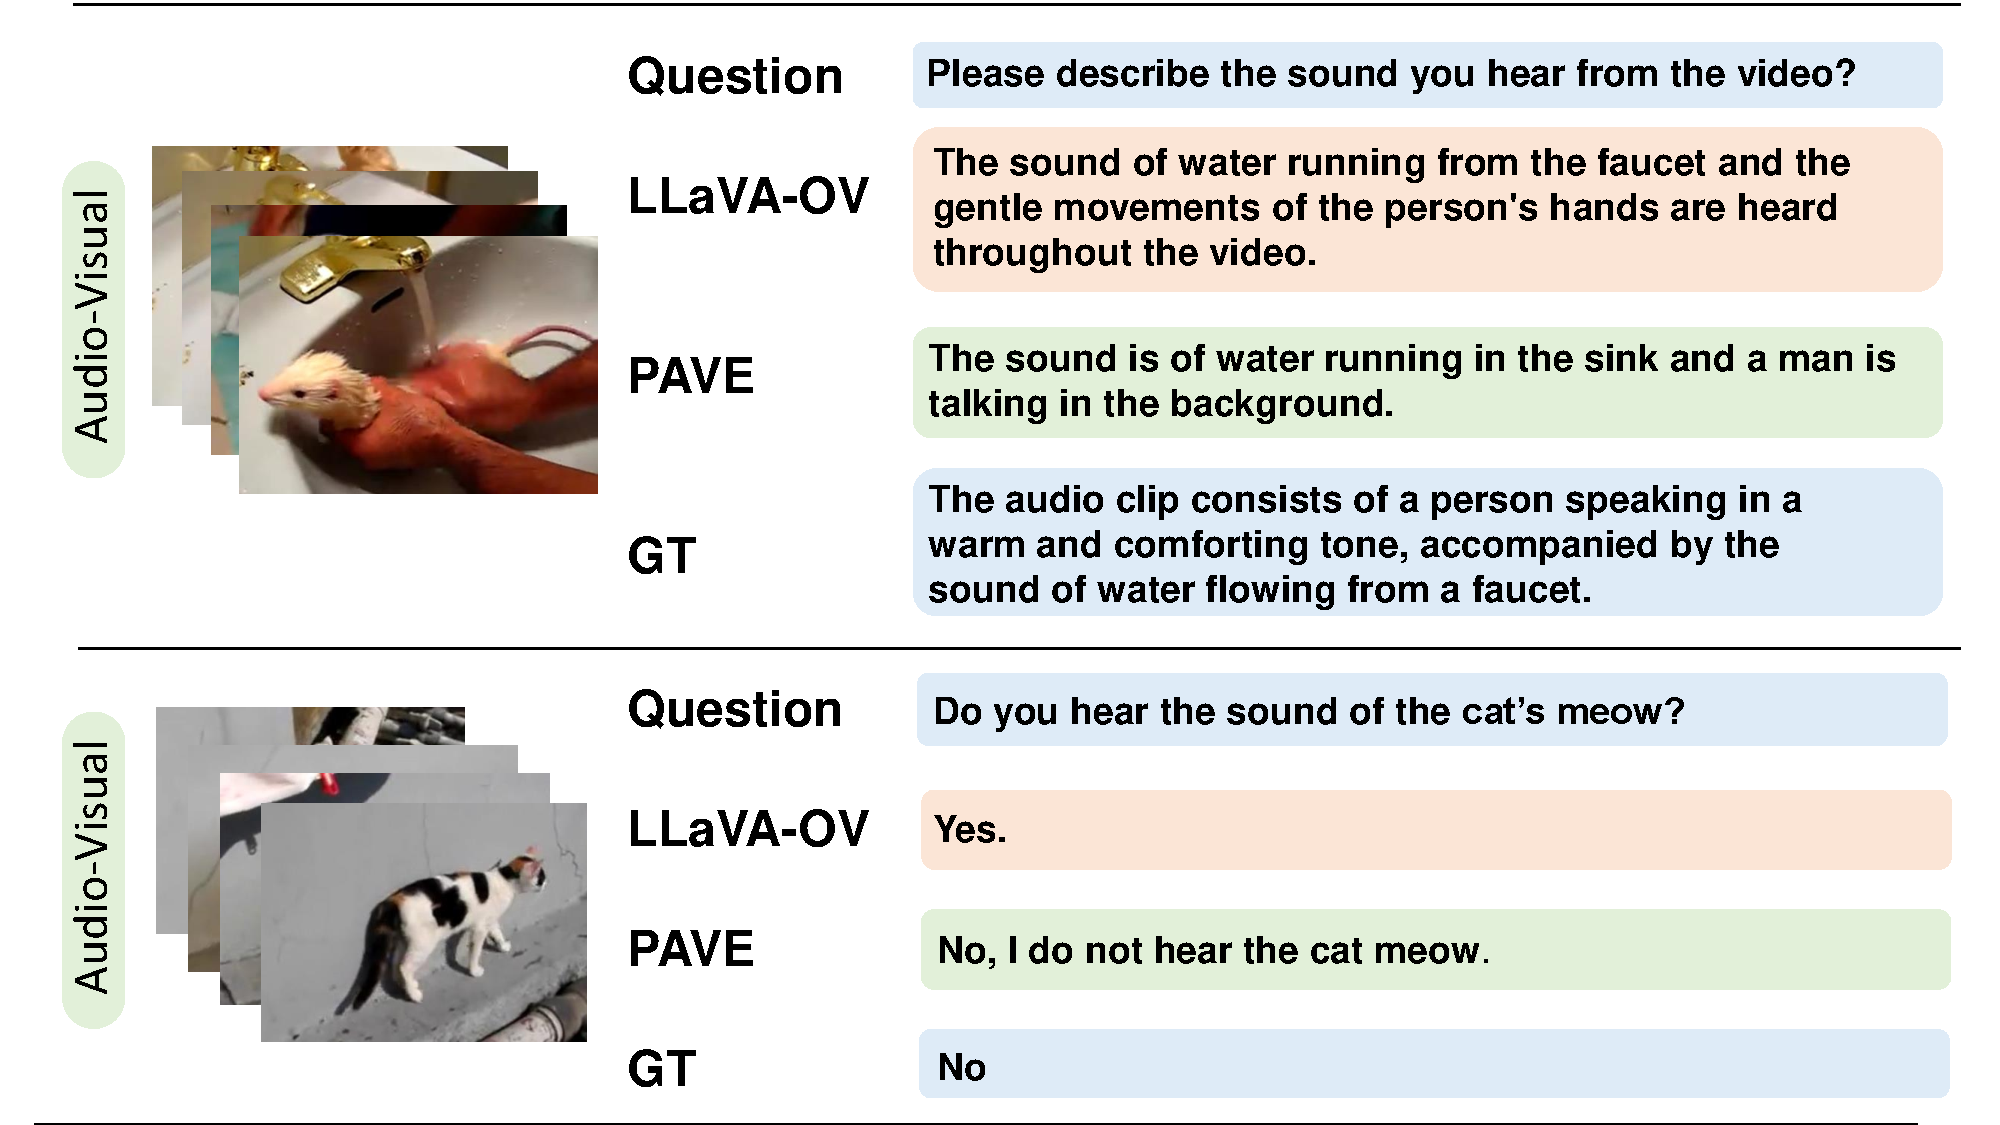
\includegraphics[width=0.8\linewidth]{figures/additional_qa_visualization.pdf}
%     % \vspace{-1em}
%     \caption{Additional visualization of audio-visual setting. We select online videos and ask question about the audio information. PAVE are able to understand the audio correctly instead of just inferring the sound from the visual information.}
%     \label{fig:additional_audio_visual}
%     % \vspace{-1em}
% \end{figure*}


\begin{figure*}[t!]
    \centering
    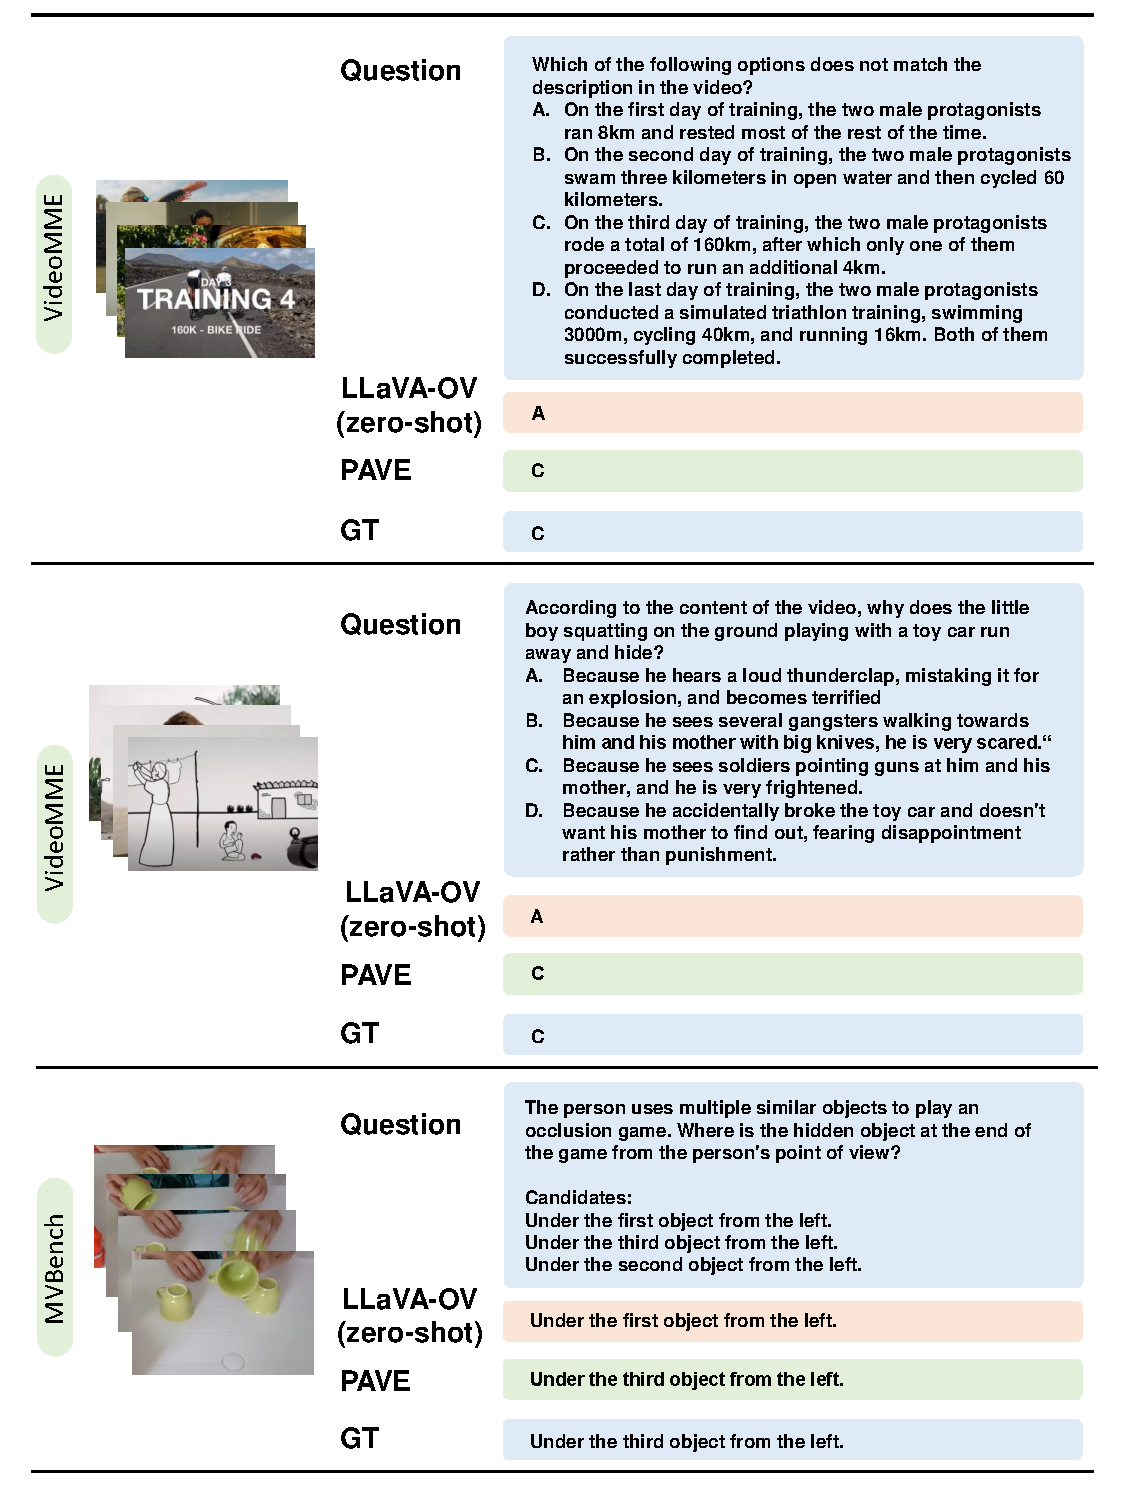
\includegraphics[width=0.75\linewidth]{figures/additional_general_qa_visualization.pdf}
    \vspace{-1em}
    \caption{Visualization of the QA results on enhanced video QA task. By making use of the video feature of the densely sampled video frames, PAVE captures more details in the video and thus improves the performance of video understanding.}
    \label{fig:enhanced_qa_visualization}
    \vspace{-1.5em}
\end{figure*}




% \section{Discussion and Future Works} \label{discussion}

% % \subsection{Discussion of training and using multiple patches}
% In the ablation study of the main paper, we investigate training multiple patches together. We provide additional experiment details and further discussion here.

% We use the enhanced video understanding patch (PAVE-7B model in Table~\ref{tab:general_video_understanding} of the main paper) in this experiment. Specifically, we employ the PAVE module from the enhanced video understanding setting and instantiate a new PAVE module with new LoRA weight for LLM to adapt the Video LLM to the setting where the audio and the densely sampled video frames serve as the side-channel information. 
% During training, we freeze the PAVE module from the enhanced video understanding setting so that the performance on the enhanced video understanding will not change while the new patch for audio-visual setting can benefit from the information in the densely sampled video frames.
% After training, we have two distinct patches: one for enhanced video understanding and another for audio-visual understanding. 
% During the inference in an audio-visual setting, we activate both patches (two PAVE modules) and the LoRA weight that was trained for the audio-visual setting. PAVE takes keyframes, high-framerate video, and audio as input.

% For the trained patches, while we can deploy them independently and regard each of them as a standalone model, we can also consider merging them into a single mixture-of-expert (MoE) model, with each task-specific patch as an expert, though this topic is already beyond the scope of this paper. This could be handled by modifying the LoRA and model wrapper to load multiple LoRA weights and PAVE modules at the same time. During inference, this MoE model routes an input to a task expert and activates its weights.
% A straightforward approach to implementing this routing mechanism is rule-based selection, where the patch is chosen based on the type of side-channel information available in a given sample. Future work could explore more advanced routing strategies that involve training the router to learn optimal patch selection.







\end{document}
